\documentclass{article}
\usepackage{iclr2027_conference,times}
\usepackage{amsmath,amssymb,booktabs,graphicx}
\usepackage{hyperref}
\usepackage{url}
\graphicspath{{figures/}}
\hypersetup{pdftitle={GNNM: Shared Propagation for Graph Neural Network Ensembles},pdfauthor={Anonymous Authors}}
% Keep \iclrfinalcopy commented out for anonymous review.
\title{GNNM: Shared Propagation for Graph Neural Network Ensembles}
\author{Anonymous Authors}
\begin{document}
\maketitle

\begin{abstract}
Graph neural network ensembles combine several predictors to improve prediction quality. We study whether members can improve their combined prediction while learning common graph weights. GNNM retains four member paths with shared propagation weights and member-specific input and output factors. Across Roman Empire, Amazon Ratings, Minesweeper, Questions and Tolokers, its recorded means exceed a four-model ensemble in 28 of 40 backbone--dataset comparisons, with positive differences for SAGE and both graph-transformer variants on every dataset. Each method uses its intended training and validation-selection procedure. A matched Roman Empire SAGE study gives a 2.94-point accuracy gain with stronger individual members despite lower disagreement. A separate internal-factor SAGE study on selected WikiCS development improves pooled accuracy despite weaker average members, with broader coverage of correct alternatives and higher calibrated negative log-likelihood than the independent ensemble. Three-seed uncertainty and reuse of development nodes limit this finding. The evidence supports sharing as a graph- and recipe-dependent prediction-quality option without identifying a general learning mechanism. Fewer stored weights are a secondary benefit, and multiple graph passes remain necessary.
\end{abstract}

\section{Introduction}
A graph neural network combines node features with information from connected nodes to make predictions. An ensemble combines several such predictors, allowing one member to compensate for another's mistakes. The purpose of a learned ensemble is to improve its combined prediction. Its members can supply correct decisions on different examples, but averaging can also discard a correct alternative. Predictive quality therefore depends on what the members learn and how their outputs combine. We study graph neural network ensembles whose members share learned propagation weights, and compare their predictions with capable independent models.

GNNM retains four prediction paths through a common graph stack. Small member-specific factors change the input and output maps, so the shared graph layers receive different hidden states and can produce different predictions. This boundary factorization uses established BatchEnsemble components \citep{wen2020batchensemble}. Related factorized models have been studied for tabular prediction \citep{gorishniy2025tabm}, and BatchEnsemble has also been applied inside GNN layers \citep{kim2023efficient}. Our contribution is an empirical study of the predictions learned under these sharing constraints. Sharing reduces stored weights, while each member still performs graph propagation; predictive quality and execution cost are measured separately.

The main benchmark covers Roman Empire, Amazon Ratings, Minesweeper, Questions and Tolokers \citep{platonov2023critical}, with eight backbones and ten official splits per dataset. Its recorded means favor GNNM over four independent ordinary models in 28 of 40 backbone--dataset comparisons. SAGE and both graph-transformer variants favor GNNM on every dataset, while other backbones include losses. The benchmark compares each method's intended training and validation-selection procedure. Separate matched studies examine sharing within a specified recipe.

Those studies show different paths to a better combined prediction. In the matched Roman Empire SAGE comparison, shared propagation improves individual members despite lower disagreement. A later internal-factor SAGE study on encountered WikiCS development instead obtains higher pooled accuracy with weaker average members and broader coverage of correct alternatives. Its calibrated negative log-likelihood remains higher than that of the genuine independent ensemble. We report the accuracy benefit and confidence tradeoff together, with capable single, joint-untied and independent-ensemble controls.

The evidence supports sharing as a prediction-quality option whose value depends on the graph, backbone and training procedure. It does not identify one general optimization mechanism or a universally preferred factor placement. The original five-dataset results remain the central benchmark; the later studies distinguish member quality, useful alternatives and pooling behavior under their own stated protocols.



\section{The GNNM model}\label{sec:method}
\paragraph{Input and member paths.}
For a graph with $n$ nodes, the input is a feature matrix $X\in\mathbb{R}^{n\times d}$ and an edge list. Each row of $X$ contains the $d$ features of one node. An input projector maps these features to $h$ hidden coordinates. GNNM creates $M$ versions of this map using a common weight matrix and short learned vectors for each member. We use $M=4$ in the main benchmark.

For any input or output projector, the member-specific operation is
\begin{equation}\label{eq:be}
\operatorname{BE}_m(U;W)=((U\odot r_m)W)\odot s_m+b_m.
\end{equation}
Here $U$ is the input to the projector, $W$ is its shared matrix, and $\odot$ means coordinatewise multiplication. The vector $r_m$ rescales input coordinates, $s_m$ rescales output coordinates, and $b_m$ adds a member-specific bias. These vectors are learned during training. A member changes the map using vectors rather than storing another full matrix.

\paragraph{Shared graph layers.}
After input projection, every member has an $n\times h$ table of hidden states. Each graph layer combines a node's state with information from its neighbors. All members use the same learned graph-layer parameters, but apply them to their own states. In attention backbones, the different states can also produce different attention coefficients. The graph layers are therefore evaluated once per member. Figure~\ref{fig:sharing} distinguishes the shared weights from the separate computations.

\begin{figure}[t]
\centering
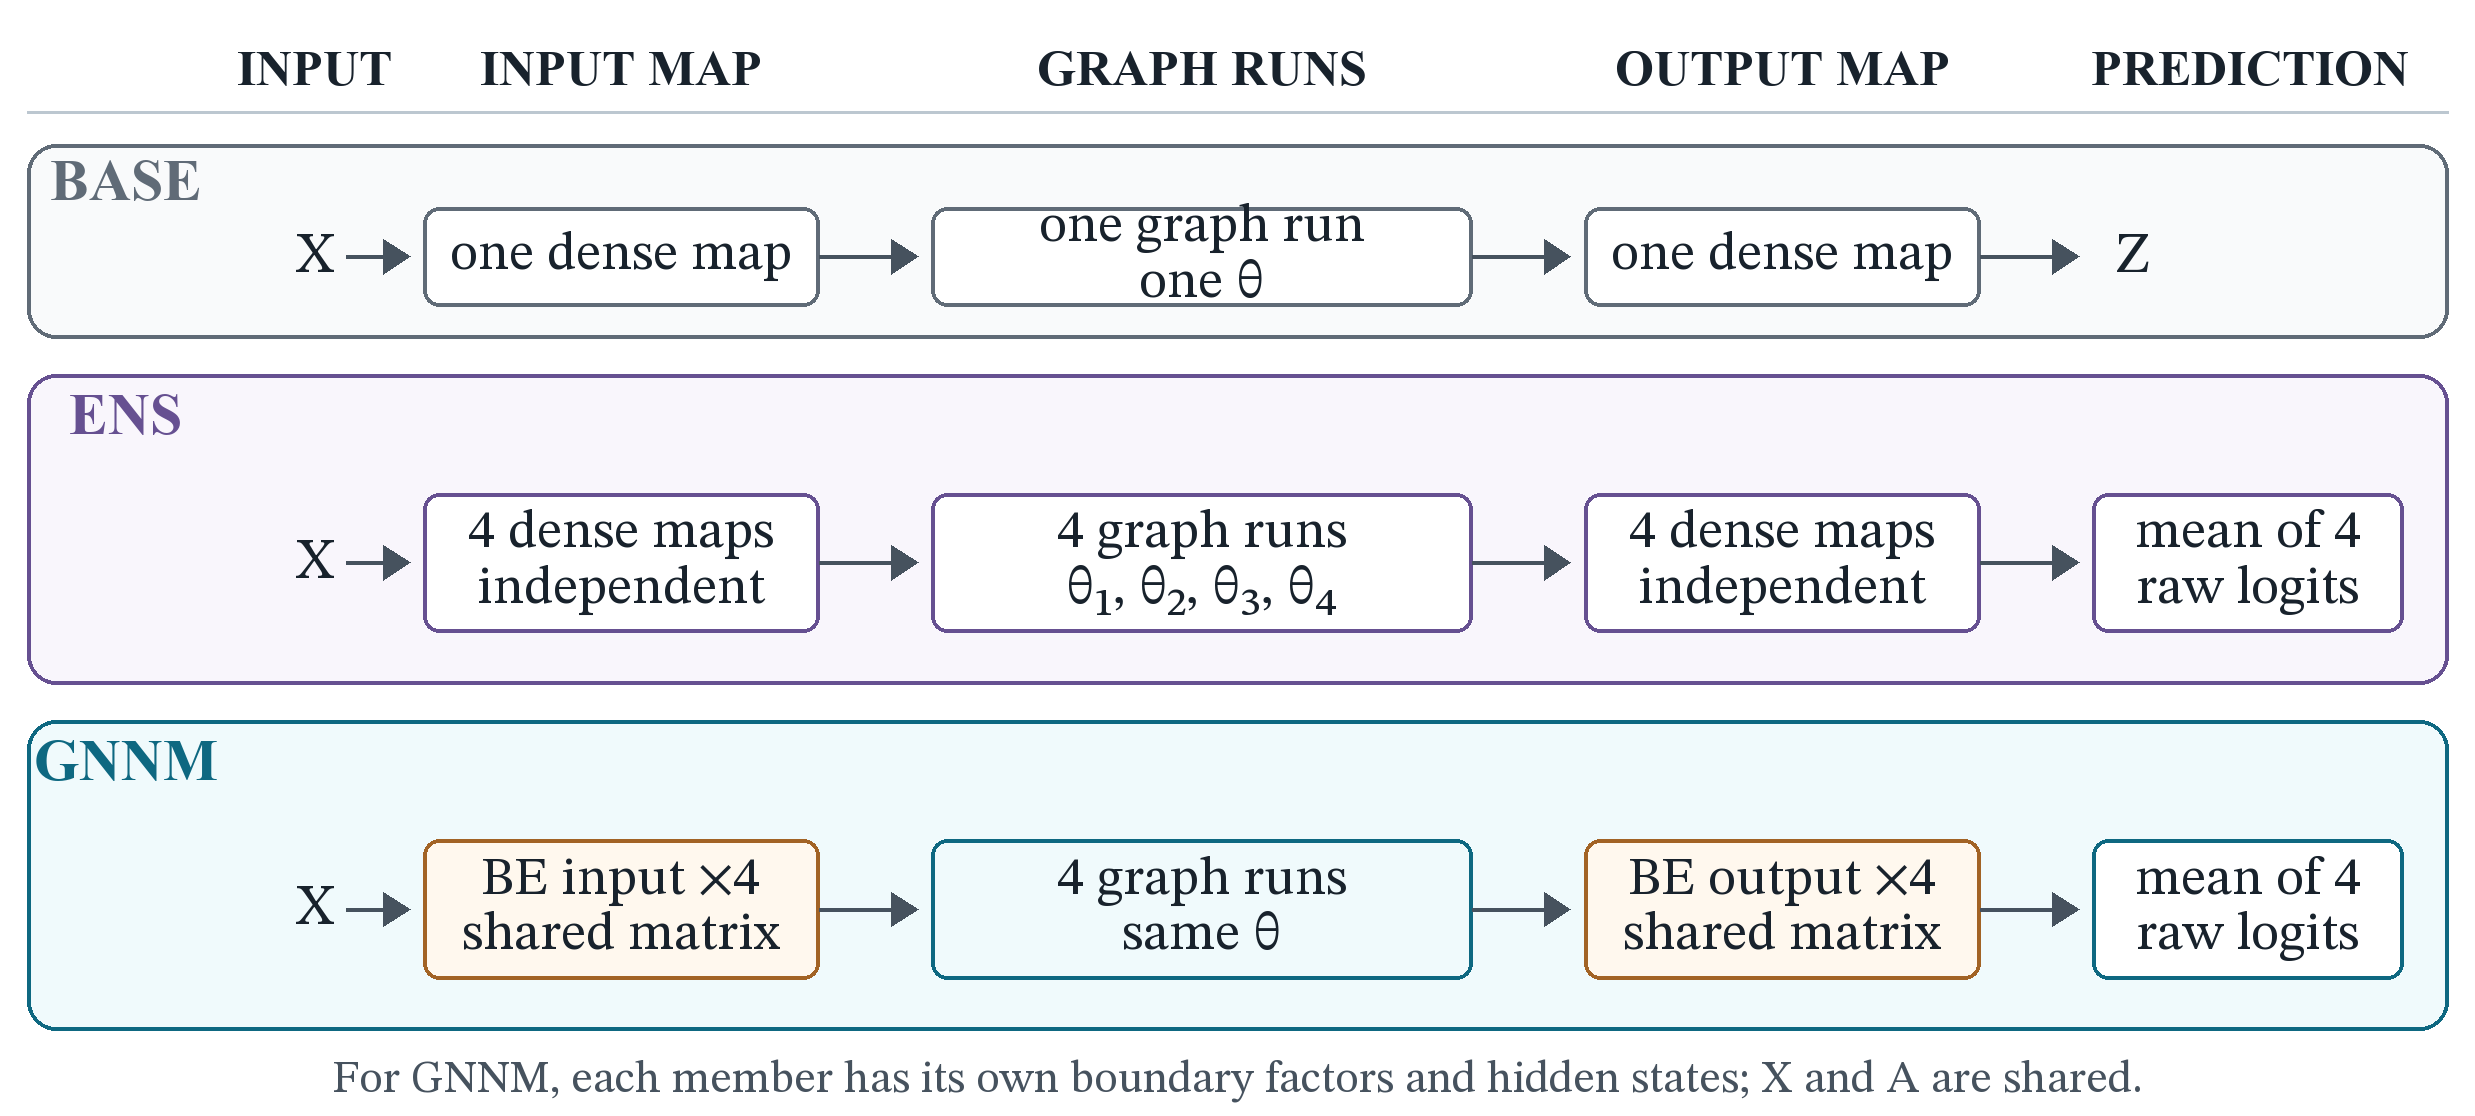
\includegraphics[width=\linewidth]{architecture_sharing_compact.png}
\caption{BASE produces one prediction. ENS stores and runs four complete models. GNNM stores one graph stack but applies it to four member-specific hidden states. The input and output matrices are each shared, with lightweight factors distinguishing the members' projectors. ENS and GNNM average the four raw output scores.}
\label{fig:sharing}
\end{figure}

\paragraph{Training and prediction.}
The output projector produces one raw score per class and node for each member. For binary tasks it produces one score. Training minimizes the average of the members' cross-entropy losses on the training nodes. Errors from all members update the common graph weights, while each member's factors also receive their own gradients. Dropout masks are drawn separately for the members.

At inference, dropout is disabled and the $M$ raw score arrays are averaged. Multiclass prediction chooses the class with the largest averaged score. For binary ROC-AUC, the averaged score ranks nodes. We average raw logits, rather than class probabilities or majority votes. The input features and graph are the same for every member. Test labels are used only to evaluate the selected predictions.

\paragraph{Stored model size.}
The input and output matrices are stored once, and the member factors grow linearly with input and hidden width. Together the two projectors contain $dh+hq+M(d+3h+2q)$ parameters, where $q$ is the output width. All graph-layer and final-normalization parameters are also stored once. An ordinary $M$-model ensemble stores $M$ complete copies. This reduces weight storage but leaves the member activations and graph computations. Appendix~\ref{app:implementation} gives initialization and the exact backbone operations.

\section{Five-dataset benchmark}\label{sec:original-benchmark}
\subsection{Experimental setup}
The benchmark uses the five datasets introduced by \citet{platonov2023critical} to evaluate learning on graphs where neighboring nodes need not share labels. Roman Empire and Amazon Ratings are multiclass tasks evaluated by accuracy. Minesweeper, Questions and Tolokers are binary tasks evaluated by ROC-AUC. Each dataset supplies ten official train/validation/test splits.

We use seven graph backbones: GCN, SAGE, GAT, GAT-sep, GT, GT-sep and TAG, plus a graph-free ResNet control. GT denotes the TransformerConv-based implementation specified in the appendix. For every backbone, BASE is one ordinary model, ENS is four independent ordinary models, and GNNM uses four member paths. This compares sharing within each architecture instead of combining different backbones into one ensemble.

All benchmark models use hidden width 512, learning rate $3\cdot10^{-5}$, AdamW with zero weight decay, LayerNorm, GELU and dropout 0.2. Depths 1--5 are evaluated, and validation chooses a depth separately for each method and official split. Runs have a 5,000-step cap and validation stopping. The supplement reconstructs the complete grid from 6,000 original run records and identifies all 1,200 selected records.

Each method uses its intended validation procedure. ENS trains its members independently and selects each member's checkpoint using its own validation score, then chooses depth using their averaged prediction. GNNM trains its four paths jointly and selects one model checkpoint using their averaged validation prediction. Both procedures use validation data to select predictions evaluated on the test split. The benchmark compares these complete methods as designed. To study the effect of shared graph weights by itself, we use separate matched comparisons below. Projector initialization also differs in the original benchmark, and its launch-time code and data fingerprints were not preserved. Appendix~\ref{app:protocol} gives the exact reconstruction rule and provenance limits.

\subsection{Predictive results}
\begin{figure}[t]
\centering
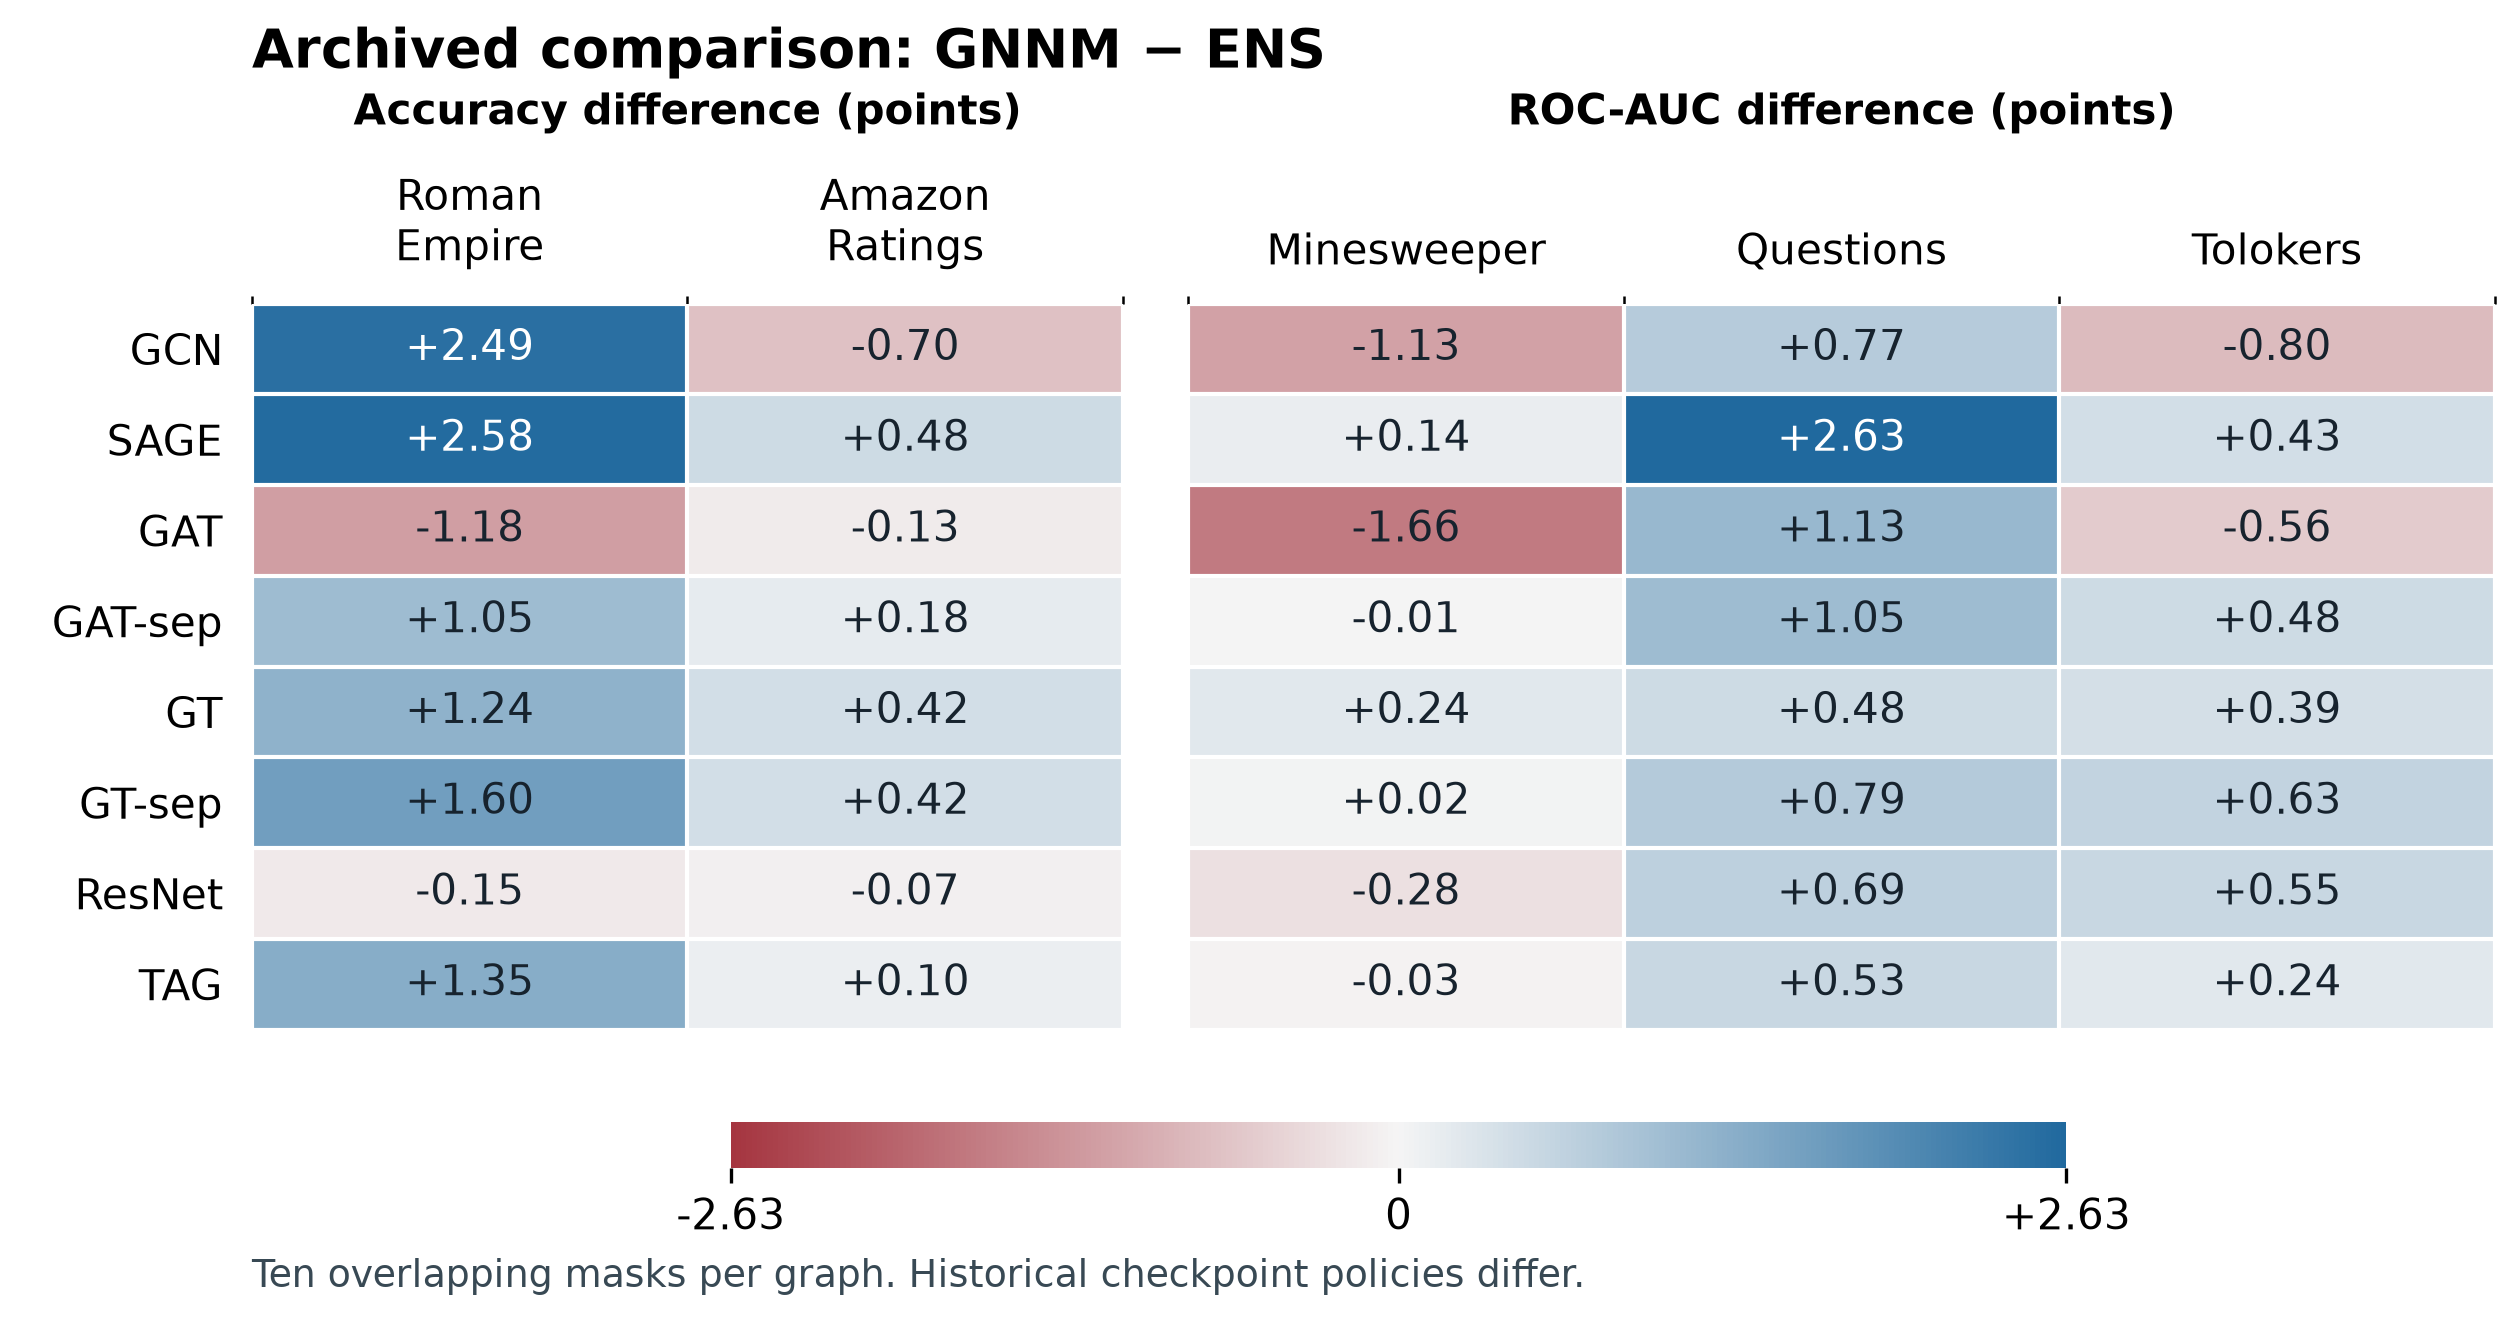
\includegraphics[width=\linewidth]{gnnm_vs_ens_heatmap.png}
\caption{GNNM minus the four-model ensemble on all five datasets and eight backbones. Each cell averages the paired differences over ten official splits, in percentage points of that dataset's metric. Blue favors GNNM and red favors ENS. The two metric families are shown separately. Each method uses its intended validation-selection rule. Appendix Table~\ref{tab:benchmark-absolute} gives all absolute scores and deviations.}
\label{fig:benchmark-main}
\end{figure}

Figure~\ref{fig:benchmark-main} shows every dataset and backbone. GNNM exceeds BASE in 33 of 40 mean comparisons and ENS in 28. Relative to ENS, it improves on six of eight backbones on Roman Empire, five on Amazon Ratings, three on Minesweeper, all eight on Questions, and six on Tolokers. These counts summarize the suite. The 40 cells share five graphs and are not 40 independent tasks.

The most consistent backbone results are SAGE, GT and GT-sep, which improve over ENS on all five datasets. For SAGE, Roman Empire rises from 87.47\% to 90.04\%, and Questions from 74.39 to 77.02 ROC-AUC points. Gains are smaller on Minesweeper and Tolokers. GAT behaves differently: it improves on Questions but loses on the other four datasets. GCN also loses on Amazon Ratings, Minesweeper and Tolokers. Sharing therefore depends on the backbone as well as the dataset.

The ResNet control ignores graph edges and improves over ENS on two datasets. Its behavior confirms that the boundary factorization can affect predictions without message passing. The graph results need additional comparisons to determine the contribution of sharing graph weights specifically. We provide those comparisons next. The appendix retains paired split differences and selection sensitivities, including the small and negative effects.

\subsection{Storage and execution cost}
In the original resource sweep, GNNM stores roughly one quarter of ENS's parameters. Its measured training-step time is 0.3--2.5\% higher. This is expected from the implementation: four different hidden-state tables still pass through the graph. Parameter storage is the measured benefit, while compute and peak memory must be assessed separately.

\begin{table}[t]
\centering\small
\setlength{\tabcolsep}{4pt}
\caption{Original resource sweep, averaged over eight backbones and five depths. Parameter counts are millions, step times are milliseconds, and peak allocation is MiB. These configurations are not necessarily the depth selected for prediction. Both methods use four paths.}
\label{tab:resource-main}
\begin{tabular}{lrrr}
\toprule
& Parameters & Step time & Peak allocation\\
Dataset & ENS / GNNM & ENS / GNNM & ENS / GNNM\\
\midrule
Roman Empire & 16.04 / 4.02 & 204.4 / 209.6 & 2228 / 2164\\
Amazon Ratings & 16.01 / 4.01 & 300.7 / 306.5 & 3706 / 3636\\
Minesweeper & 15.40 / 3.86 & 126.8 / 128.5 & 1679 / 1543\\
Questions & 16.00 / 4.01 & 542.1 / 552.8 & 6385 / 6420\\
Tolokers & 15.41 / 3.86 & 658.7 / 660.6 & 12953 / 12818\\
\bottomrule
\end{tabular}
\end{table}

Table~\ref{tab:resource-main} separates these costs. The sweep uses 50 warmup steps and 200 synchronized optimization steps. It processes members sequentially and uses weight decay 0.01 for all methods, whereas predictive runs use zero decay. The original sweep records do not independently identify the device model. Later profiles use an identified A100 and saved timing samples. Appendix~\ref{app:cost-details} gives the protocols and full measurements. We do not claim lower latency or lower peak memory from fewer stored parameters.

\section{Analysis of the member paths}\label{sec:analysis}
The benchmark measures the complete GNNM recipe, which changes both the projectors and the sharing of graph weights. To examine the contribution of sharing itself, we start with GNNM and give each member its own copy of the graph stack. The copies initially contain the same values, so the member functions are matched before training. During training, the copies can change independently. Both versions choose a checkpoint using the same averaged validation prediction. Their difference measures what happens when the requirement to share graph weights is removed, under this training recipe.

We make this comparison on a favorable benchmark setting: five-layer SAGE, width 512, on Roman Empire masks 0--4. Every four-member method in Table~\ref{tab:component-main} uses the common checkpoint rule. The setting was chosen after the benchmark, so the study examines one observed success. It does not estimate the effect of sharing across new graphs.

\begin{table}[t]
\centering\small
\setlength{\tabcolsep}{5pt}
\caption{Roman Empire component study. Accuracy is mean $\pm$ standard deviation over five overlapping official masks. All four-member rows use a pooled checkpoint rule. The first two rows form the matched-initialization sharing comparison. The remaining component comparisons have the initialization relationships specified in Appendix~\ref{app:controls}.}
\label{tab:component-main}
\begin{tabular}{lrr}
\toprule
Method & Accuracy (\%) & Parameters ($10^6$)\\
\midrule
GNNM & $89.50\pm0.29$ & 6.738\\
Private propagation for every member & $86.56\pm0.57$ & 26.437\\
\midrule
Four ordinary models (pooled ENS) & $87.52\pm0.26$ & 26.923\\
Four independent input/output maps & $86.99\pm0.38$ & 7.221\\
Input factors only & $89.35\pm0.32$ & 6.736\\
Output factors only & $84.96\pm0.47$ & 6.733\\
Four output heads & $84.97\pm0.56$ & 6.758\\
Frozen output factors & $89.48\pm0.28$ & 6.736\\
Factors also inside graph layers & $89.66\pm0.14$ & 6.871\\
One-member GNNM & $85.47\pm0.64$ & 6.732\\
BASE & $86.21\pm0.47$ & 6.731\\
\bottomrule
\end{tabular}
\end{table}

GNNM exceeds the version with private graph stacks by 2.94 accuracy points on average, with positive differences on all five masks. It also exceeds the ordinary ensemble under the common checkpoint rule by 1.99 points. The private-stack model can reproduce any GNNM prediction by keeping its four graph stacks identical. GNNM's higher accuracy here therefore cannot come from access to a larger set of prediction functions. It concerns what this training and checkpoint-selection procedure finds under the sharing constraint. Giving members private weights changes both capacity and optimizer histories, which this comparison does not separate. Repeating the matched sharing comparison on mask 0 with three optimization seeds gives a gain of $3.33\pm0.63$ points (sample SD), positive for every seed. This remains evidence from one graph and a finite training budget.

Sharing weights is only part of GNNM: its members also enter the graph layers with different hidden states. To examine this distinction, we compare varying the input map with varying only the output map. The latter makes several predictions from one common propagated representation. The input-only variant scores close to GNNM, whereas output-only and heads-only variants score lower in this case. Freezing the output factors barely changes the mean, while adding factors inside every graph layer gives a small increase. This pattern is consistent with useful input variation in this setting. Several variants start from different functions, so these comparisons do not isolate a single component or establish that both boundary projectors are necessary or optimal.

A higher ensemble score can arise because its members become more accurate, because averaging corrects more of their errors, or both. We therefore return to the saved predictions from the matched sharing comparison. For each method, we calculate the mean accuracy of its four members and then the additional accuracy obtained by averaging their raw scores. This divides the observed ensemble difference into two quantities without changing any predictions.

For the Roman SAGE comparison, GNNM's members are 3.08 points more accurate than the untied members on average. Its gain from averaging is 0.14 points smaller. Together these changes give the 2.94-point pooled advantage. Pairwise class disagreement falls from 8.00\% to 6.07\%. Thus this favorable result comes from better members despite lower measured disagreement. More disagreement alone is not a sufficient explanation of ensemble quality.

A parallel comparison with Roman GAT checks whether this SAGE pattern also appears in an attention backbone. The mean shared-minus-private difference is only 0.04 points, with mixed signs across masks. The original GAT losses therefore do not reproduce as a large penalty from sharing in this case. Together, these results locate a favorable SAGE effect and prevent its member-accuracy explanation from being applied to every backbone. They describe the selected predictions, without establishing why training finds them. Appendix~\ref{app:gat-pair} gives the GAT masks and decision counts.

\section{Internal SAGE sharing under stronger references}\label{sec:internal-sage}
This study examines whether a shared bank produces better combined predictions than capable single models and complete ensembles. It extends factor placement into the native SAGE stack and evaluates the resulting training procedures on encountered WikiCS development. It is separate from the original five-dataset benchmark and the Roman component study.

The internal version places input and output factor vectors around every native dense map, including the input/output projectors, SAGE projections and feed-forward maps. Shared matrices and native biases remain trainable and retain their original initialization; private factor vectors distinguish four routes. The first input factors start with independent signs, and later factors start at one. Each route receives its own persistent dropout stream and makes a complete native graph pass. Unlike the original boundary projectors in Section~\ref{sec:method}, this version retains the shared native bias and also changes the internal maps. Factor placement, initialization and bias are therefore distinct parts of the recipe.

The fixed configuration uses two residual SAGE blocks, hidden width 128, LayerNorm, dropout 0.2 and AdamW with learning rate 0.001 and zero decay. Training minimizes mean ordinary member cross-entropy, with no pooled-loss gradient or context auxiliary. Prediction averages member class probabilities. Checkpoints maximize pooled development accuracy, retaining the earliest strict maximum, with a 1,000-update ceiling and 300-update stale patience.

The matched joint untied bank gives each route a complete private body. Its initial route functions, factor/dropout starts, mean-member objective and coherent pooled checkpoint selection match the shared bank. The genuine factorized independent ensemble has four complete bodies with separate native starts, optimizers, unscaled own losses and own checkpoint selectors, followed by probability averaging. Ordinary and factorized singles retain their own full losses and selectors. These five arms compare complete acquisition procedures; their parameter ownership and optimization histories differ.

All results below are means over three paired optimizer seeds on the same 5,274 development nodes used for checkpoint selection. Fixed five-fold temperature calibration follows native selection. These selected development readouts do not provide unused whole-pipeline confirmation.

Figure~\ref{fig:internal-members-coverage} shows all five arms; Appendix Table~\ref{tab:internal-sage-F} gives their absolute scores and confidence metrics. The shared bank gains 0.720516 percentage points over matched joint untied4 and 0.537227 points over genuine factorized I4, with positive differences at every seed. It also gains 1.301985 points over the ordinary single and 1.491594 over the factorized single. Descriptive paired-seed 95\% intervals are $[0.2712,1.1698]$ points versus joint untied4 and $[-0.2653,1.3398]$ versus I4; they condition on this setting and do not account for selection or variability across graphs.

\begin{figure}[t]
\centering
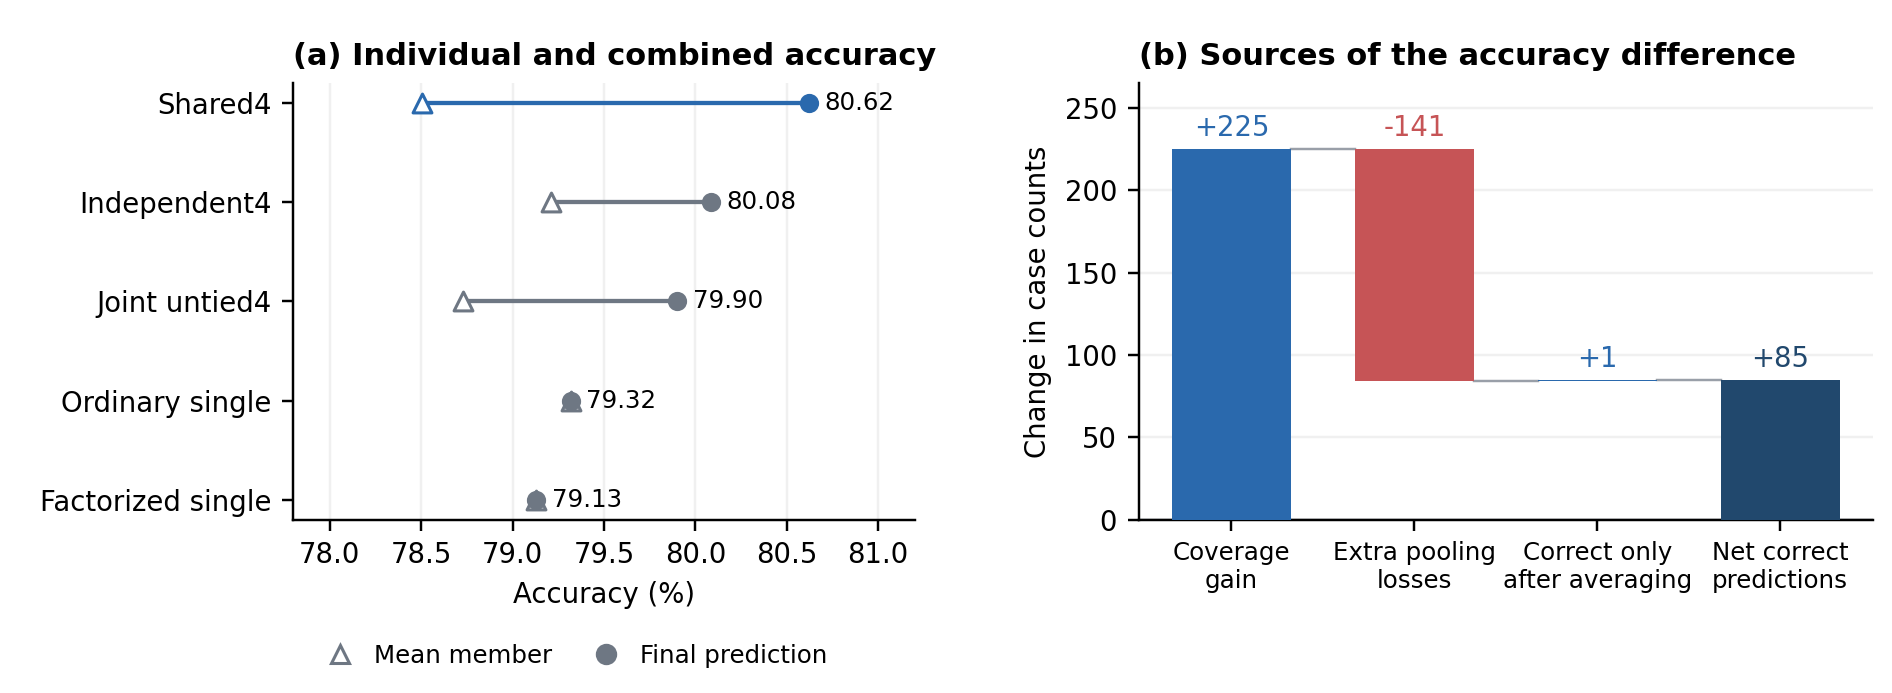
\includegraphics[width=\linewidth]{F_member_coverage_v2.png}
\caption{Internal SAGE on selected WikiCS development. (a) Shared4's average member is weaker than either complete ensemble control, while its combined prediction is more accurate. Both single-model references are shown. (b) Against independently acquired factorized models, 225 added covered cases are offset by 141 extra losses during averaging; one aggregation-only correction leaves 85 more correct decisions. Counts repeat the same 5,274 nodes across three optimizer seeds. The paired mean accuracy gain is 0.537 points, with a descriptive 95\% interval of $[-0.265,1.340]$; this is not unused confirmation or a statistically established superiority claim. Calibrated NLL is higher than that of the independent ensemble.}
\label{fig:internal-members-coverage}
\end{figure}


Shared4 has higher calibrated NLL than both ensemble controls, while calibrated Brier favors Shared4 over both. The accuracy benefit therefore accompanies a probability-quality tradeoff that differs across proper scores. Appendix~\ref{app:internal-sage-F} gives the absolute confidence metrics and the study's predeclared decision rules.

Coverage counts nodes with at least one correct member. A covered alternative can still be lost when the member probabilities are averaged. Across the three repeated readouts, Shared4 covers 13,731 cases versus 13,447 for joint untied4 and 13,506 for I4. It loses 976 of its covered cases in pooling, versus 805 and 835 for those controls. Shared4 also supplies one aggregation-only correction, leaving 114 and 85 more correct pooled decisions, respectively. Direct paired repairs/harms are 671/557 versus joint untied4 and 645/560 versus I4.

Shared4's members are less accurate on average than either ensemble control, yet the served bank is more accurate. This differs from the matched Roman SAGE result, where stronger members account for the gain. The two observations support reporting member quality and useful alternatives together. Their repeated-node counts are descriptive; they do not identify error covariance or establish a general cause of the learned differences.

Fewer stored weights remain a secondary benefit: Shared4 has 216,674 parameters, versus 832,256 for the complete four-body controls. Its recorded acquisition sum is 71.676 seconds, versus 50.025 for joint untied4 and 58.620 for I4. These scopes include different stopping histories and do not establish lower latency. Full seed, confidence, error and cost records accompany the study.



\section{Scope across sharing placements and budgets}\label{sec:additional}
An ordinary ensemble can also store fewer weights by making each member narrower. A useful storage comparison must therefore give this smaller ensemble a similar parameter budget. On Roman SAGE, we choose its width by parameter count before scoring: four width-256 models contain 6.908 million parameters, close to width-512 GNNM's 6.738 million. GNNM scores 89.50\% versus 88.14\%, but inference takes 109.7 ms versus 39.9 ms. In this setting, sharing allows wider member states and higher accuracy within a similar weight budget, at the cost of longer computation. A wider single model chosen by training-step time also scores lower, although its complete training finishes sooner (Appendices~\ref{app:param-matched} and~\ref{app:strong-base}).

Additional two-block SAGE studies compare full sharing with variants having one private graph block, either first or last, under validation-selected optimizer settings. Full sharing improves only WikiCS in the four-graph primary grid. Selected partial sharing nearly ties ENS on raw Cora, improves WikiCS, and loses on Actor and filtered Chameleon (Tables~\ref{tab:tuned-cora}--\ref{tab:tuned-chameleon-filtered}). It also loses on CiteSeer and PubMed (Tables~\ref{tab:confirmation-citeseer} and~\ref{tab:confirmation-pubmed}); normalizing Cora's features changes its outcome (Tables~\ref{tab:cora-raw} and~\ref{tab:cora-normalized}).

At similar stored-weight budgets, selected private-last models improve WikiCS and normalized Cora with higher measured inference latency (Tables~\ref{tab:wikics-matched-budget} and~\ref{tab:cora-matched-budget}). These graph, placement and preprocessing choices followed earlier outcomes. Appendix~\ref{app:sharing-scope-summary} summarizes the numerical contrasts and limits; Appendix~\ref{app:validation-tuning} gives the full optimizer protocol. No rule for choosing sharing on a new graph has been validated independently.

\section{Related work}
Deep ensembles train and average independent predictors \citep{lakshminarayanan2017simple}. TreeNets share early computation before branching \citep{lee2015heads}. GNNM instead creates distinct member states before graph propagation and shares the weights applied to those states. BatchEnsemble provides the multiplicative factorization \citep{wen2020batchensemble}, and TabM studies related models for tabular data \citep{gorishniy2025tabm}. Kim's master's thesis applies BatchEnsemble inside GNN layers \citep{kim2023efficient}. Its bibliographic record is supplied, and our added-factor comparison is not an exact reproduction of that implementation.

Other approaches target different costs. GEENI approximates constituent GNNs to reduce ensemble latency \citep{nagarajan2022geeni}, and ensembles can be distilled into one predictor \citep{zhang2024e2gnn}. Graph mixtures learn how to choose or weight experts \citep{wang2023graph,deng2025mixture}, whereas GNNM uniformly averages member scores. MIMO trains multiple predictions within one forward pass \citep{havasi2021training}, while Packed-Ensembles use grouped operations to run structured ensembles together \citep{laurent2023packed}. These are relevant alternatives that we have not compared empirically. Our experiments do not establish a ranking against every efficient ensemble method. The supplement gives the tested alternatives, including a local MC Dropout comparison, and documents their scope.

\section{Limitations and conclusion}
The original five-dataset benchmark favors GNNM most consistently for SAGE and the two graph-transformer variants, while other backbones include losses. The matched Roman SAGE comparison locates a quality gain through stronger individual members. The internal SAGE development comparison shows a different pattern: broader correct-alternative coverage offsets weaker average members and more pooling losses. Its raw accuracy advantage over capable ensembles accompanies higher calibrated NLL. These findings support evaluating sharing by the combined prediction and its probability quality, without identifying a universal optimization mechanism or factor placement.

The historical benchmark compares intended selection procedures and has incomplete launch-time source/data fingerprints. Follow-up studies were motivated by earlier outcomes; the internal-SAGE result uses the same development nodes for native selection and subsequent calibration. Overlapping graph splits and a few optimizer seeds do not establish an average effect across unseen graph tasks. Additional sharing placements and budgets include failures, and some selected checkpoints remain late in training. Stored-weight savings do not eliminate repeated graph computation or imply lower latency. Prediction quality, confidence and measured costs therefore retain separate scopes.

\section*{Reproducibility statement}
The appendix specifies model definitions, optimization and checkpoint-selection rules, complete benchmark scores and internal-SAGE development outcomes. The accompanying code and evidence supplement records run results, validation traces, selection locks and selected predictions. Historical launch-time model-source, environment and exact data fingerprints are incomplete, preventing exact replay of the original benchmark training runs.

\section*{AI use statement}
OpenAI Codex was used during earlier research and manuscript preparation for literature search, editing, draft critique, the architecture figure, experimental implementation and data preparation, and artifact audits. The authors checked numerical claims against preserved run records or completed experiments and are responsible for the final text, code, analyses and citations.

\bibliographystyle{iclr2027_conference}
\bibliography{references}
\clearpage
\appendix
\renewcommand{\thesection}{A\arabic{section}}
\renewcommand{\theHsection}{appendix.\arabic{section}}
\renewcommand{\thefootnote}{\arabic{footnote}}
% Historical appendix content is preserved once; subsequent fragments add scoped evidence.
\section*{Appendix guide}
This appendix records the exact model, selection rules, per-setting results,
resource measurements, and provenance limits. All tables report the stated
repeated unit: seeds on one split or official masks on one graph. Neither is a
sample of independent graph tasks. The accompanying anonymous code supplement
holds the complete validation matrices, selected records, prediction
artifacts, source hashes, and verifiers; the compact upload does not include
all trained checkpoints. The paper and this appendix form one submission PDF.

\section{Method, implementation, and exact scope}\label{app:implementation}
The input and output BatchEnsemble projectors use shared bias-free matrices
with Xavier-uniform initialization. An input factor $r_m$ starts with
independent equiprobable signs; its output scale starts at one and bias at
zero. All output-projector factors start at identity scale and zero bias.
Input-projector output receives dropout $0.2$ and GELU. LayerNorm precedes
the output projector. Four member losses are averaged during training;
raw member logits are averaged for checkpoint selection and inference.
Multiclass tasks use cross-entropy and binary tasks use binary
cross-entropy with logits. Each member propagates a distinct hidden state.

The supplied implementation uses external residual blocks at hidden width
$h$. Let $D$ be dropout $0.2$ and let $F_k(z)=D(A_2(\operatorname{GELU}(D(A_1(z)))))$,
where $A_1:\mathbb R^{kh}\to\mathbb R^h$ and
$A_2:\mathbb R^h\to\mathbb R^h$ are biased learned maps. With
$u=\operatorname{LayerNorm}(h)$, ResNet sets $h'=h+F_1(u)$ and has
\emph{no graph operation}. GCN, GAT, and TAG set
$h'=h+F_1(C(u))$; SAGE and GAT-sep set
$h'=h+F_2([u,C(u)])$. Here $C$ is the corresponding PyTorch Geometric
convolution \citep{kipf2017semi,hamilton2017inductive,velickovic2018graph,du2017topology,brody2022how,fey2019pyg}.
TAG uses three hops. GT and GT-sep use a TransformerConv residual
addition, followed by a separate $F_1$ residual addition
\citep{shi2021masked}. GT projects the convolution output with an
$h\to h$ map; GT-sep projects its concatenation with $u$ using a
$2h\to h$ map. At width 512, attention variants have eight heads and coefficient dropout
$0.2$. GT variants also use TransformerConv's internal root skip. The original benchmark width is
512; the primary matched SAGE study uses width 128. In the historical loader, added self-loops are not added a second time
by the configured convolutions. The newer SAGE grid adds no self-loops.
These equations describe the supplied code; historical launch-time
model-source hashes were not retained.

BASE uses ordinary dense projectors with PyTorch default initialization
and bias. An $M=1$ BatchEnsemble model therefore is not an exactly
initialization-matched BASE. A four-member explicit ensemble can represent
every deterministic GNNM inference function by copying the common graph
weights into four ordinary models and replacing each boundary projector
with its member's effective dense map. This inclusion concerns function
representation and says nothing about what training finds.

\section{Equal-grid node comparisons and matched sensitivities}\label{app:validation-tuning}
The primary four-graph grid covers public Cora, WikiCS split 0, Actor
split 0, and official filtered Chameleon split 0. We retain source
features and masks, coalesce and symmetrize edges, and add no self-loops.
Symmetrizing filtered Chameleon changes its directed-edge convention.
TIED denotes GNNM with all graph blocks shared. UNTIED retains the
boundary projectors but makes every graph block private. The two partial
variants make only the first or last block private. Each arm has two
residual SAGE blocks, width 128, LayerNorm and dropout
$0.2$. BASE and ENS use ordinary initializations. TIED, private-first,
private-last and UNTIED copy a canonical projector initialization, match
post-construction random-generator states, and pass a numerical initial
member-logit check. Private-first and private-last store equal numbers
of parameters. UNTIED copies both graph blocks for every member.

Every graph--arm pair receives learning rates
$\{0.0003,0.001,0.003\}$ crossed with AdamW decay $\{0,0.01\}$.
Three seeds and exactly 1,000 full epochs give $4\cdot6\cdot6\cdot3=432$
planned cells. A nonfinite seed invalidates its three-seed candidate.
Whole-model checkpoints maximize pooled validation accuracy, then
minimize validation cross-entropy, then choose the earliest epoch. Each
arm's six candidates are ranked by mean selected validation accuracy,
mean cross-entropy, lower learning rate and lower decay. Both partial
placements receive the complete six-candidate search before one is
chosen by validation; that family has twice the configuration search
of ENS. The complete validation grid was audited and locked before
selected/default test scoring. The default is learning rate $0.001$,
zero decay. All 141 allowed selected/default score records and the
original float32 selected test member logits are in the supplement.
The three seeds quantify optimization variation on a single published
split. Graphs were chosen after earlier work and are not untouched
holdouts. Cora and WikiCS used the original A100 runtime; Actor and
filtered Chameleon used a second A100 runtime. Within-graph arms share
a runtime, while exact equality of software stacks across hosts is not
claimed. Selected epochs near the cap limit convergence claims.

\begin{table}[t]
\centering
\caption{Validation-tuned comparison on Cora. Test accuracy is mean $\pm$ sample standard deviation over three optimization seeds on one published split. Every arm receives six optimizer candidates. Default uses learning rate 0.001 and zero decay. The star marks the partial placement chosen using validation, after tuning both partial arms (12 configurations). Parameters are in millions.}
\label{tab:tuned-cora}
\small
\setlength{\tabcolsep}{4pt}
\begin{tabular}{lrrrrrr}
\toprule
Arm & LR & Decay & Val. (\%) & Test (\%) & Default (\%) & Params\\
\midrule
BASE & 0.001 & 0.01 & 70.933 & $71.167 \pm 0.404$ & 71.200 & 0.349831\\
ENS & 0.0003 & 0.01 & 72.533 & $73.600 \pm 0.400$ & 73.233 & 1.399324\\
TIED & 0.001 & 0.01 & 67.400 & $67.700 \pm 2.524$ & 67.733 & 0.357020\\
Private first$^{\star}$ & 0.003 & 0 & 73.533 & $73.667 \pm 1.021$ & 72.967 & 0.604700\\
Private last & 0.003 & 0.01 & 71.800 & $70.833 \pm 2.732$ & 72.867 & 0.604700\\
UNTIED & 0.003 & 0 & 72.867 & $73.633 \pm 0.289$ & 72.567 & 0.852380\\
\bottomrule
\end{tabular}
\end{table}

\begin{table}[t]
\centering
\caption{Validation-tuned comparison on WikiCS. Test accuracy is mean $\pm$ sample standard deviation over three optimization seeds on one published split. Every arm receives six optimizer candidates. Default uses learning rate 0.001 and zero decay. The star marks the partial placement chosen using validation, after tuning both partial arms (12 configurations). Parameters are in millions.}
\label{tab:tuned-wikics}
\small
\setlength{\tabcolsep}{4pt}
\begin{tabular}{lrrrrrr}
\toprule
Arm & LR & Decay & Val. (\%) & Test (\%) & Default (\%) & Params\\
\midrule
BASE & 0.003 & 0.01 & 80.724 & $77.977 \pm 0.526$ & 78.143 & 0.205194\\
ENS & 0.003 & 0.01 & 81.440 & $78.867 \pm 0.121$ & 78.736 & 0.820776\\
TIED & 0.001 & 0.01 & 82.231 & $79.038 \pm 0.528$ & 79.043 & 0.207872\\
Private first & 0.001 & 0.01 & 81.967 & $78.610 \pm 0.366$ & 78.610 & 0.455552\\
Private last$^{\star}$ & 0.001 & 0 & 82.514 & $79.608 \pm 0.195$ & 79.608 & 0.455552\\
UNTIED & 0.001 & 0.01 & 81.948 & $79.043 \pm 0.294$ & 79.055 & 0.703232\\
\bottomrule
\end{tabular}
\end{table}

\begin{table}[t]
\centering
\caption{Validation-tuned comparison on Actor. Test accuracy is mean $\pm$ sample standard deviation over three optimization seeds on one published split. Every arm receives six optimizer candidates. Default uses learning rate 0.001 and zero decay. The star marks the partial placement chosen using validation, after tuning both partial arms (12 configurations). Parameters are in millions.}
\label{tab:tuned-actor}
\small
\setlength{\tabcolsep}{4pt}
\begin{tabular}{lrrrrrr}
\toprule
Arm & LR & Decay & Val. (\%) & Test (\%) & Default (\%) & Params\\
\midrule
BASE & 0.003 & 0.01 & 37.185 & $37.193 \pm 1.396$ & 36.228 & 0.285445\\
ENS & 0.003 & 0.01 & 38.268 & $37.632 \pm 0.648$ & 37.610 & 1.141780\\
TIED & 0.003 & 0.01 & 37.760 & $36.469 \pm 0.790$ & 37.303 & 0.290616\\
Private first$^{\star}$ & 0.003 & 0.01 & 38.144 & $37.193 \pm 1.096$ & 36.645 & 0.538296\\
Private last & 0.003 & 0.01 & 38.021 & $37.522 \pm 0.428$ & 37.522 & 0.538296\\
UNTIED & 0.003 & 0.01 & 38.062 & $36.447 \pm 0.863$ & 37.390 & 0.785976\\
\bottomrule
\end{tabular}
\end{table}

\begin{table}[t]
\centering
\caption{Validation-tuned comparison on official filtered Chameleon. Test accuracy is mean $\pm$ sample standard deviation over three optimization seeds on one published split. Every arm receives six optimizer candidates. Default uses learning rate 0.001 and zero decay. The star marks the partial placement chosen using validation, after tuning both partial arms (12 configurations). Parameters are in millions.}
\label{tab:tuned-chameleon-filtered}
\small
\setlength{\tabcolsep}{4pt}
\begin{tabular}{lrrrrrr}
\toprule
Arm & LR & Decay & Val. (\%) & Test (\%) & Default (\%) & Params\\
\midrule
BASE & 0.0003 & 0.01 & 42.393 & $37.113 \pm 2.247$ & 37.973 & 0.463749\\
ENS & 0.001 & 0.01 & 46.225 & $41.924 \pm 2.543$ & 41.924 & 1.854996\\
TIED & 0.001 & 0.01 & 44.832 & $37.113 \pm 0.515$ & 38.832 & 0.474492\\
Private first & 0.003 & 0.01 & 42.276 & $39.347 \pm 2.146$ & 39.863 & 0.722172\\
Private last$^{\star}$ & 0.003 & 0.01 & 43.554 & $38.832 \pm 3.274$ & 39.691 & 0.722172\\
UNTIED & 0.003 & 0.01 & 42.509 & $36.082 \pm 2.362$ & 41.409 & 0.969852\\
\bottomrule
\end{tabular}
\end{table}

\subsection{Paired decisions and additional graphs}\label{app:paired-decisions}
For the validation-selected partial placement versus selected ENS, each
test node and seed belongs to one of four mutually exclusive groups:
both correct, partial only correct, ENS only correct, or neither correct.
The signed accuracy difference is the difference between the two
exclusive counts divided by the number of seed--node decisions. Counts
show where a score difference comes from; reused nodes and seeds are not
independent observations, so no node-level significance test is used.

\begin{table}[t]
\centering\small
\caption{Illustrative paired optimizer-seed intervals for selected partial sharing minus selected ENS. Each row uses three paired seeds on one fixed graph split. The interval is the mean plus or minus $t_{0.975,2}\,\mathrm{SD}/\sqrt{3}$, with $t_{0.975,2}=4.30265$. It assumes independent approximately normal optimizer-seed differences and conditions on the frozen setting. Candidate selection used these seeds' validation outcomes, which this calculation does not account for. These are not intervals over graph tasks or nodes, or simultaneous intervals.}
\label{tab:conditional-seed-intervals}
\setlength{\tabcolsep}{4pt}
\begin{tabular}{lrrl}
\toprule
Setting & Mean $\Delta$, pp & SD, pp & Conditional 95\% interval, pp\\
\midrule
Primary Cora raw & $+0.067$ & 1.041 & $[-2.519,+2.652]$\\
Primary WikiCS & $+0.741$ & 0.240 & $[+0.146,+1.336]$\\
Primary Actor & $-0.439$ & 1.259 & $[-3.567,+2.689]$\\
Filtered Chameleon & $-3.093$ & 5.809 & $[-17.523,+11.338]$\\
CiteSeer & $-1.833$ & 1.168 & $[-4.734,+1.067]$\\
PubMed & $-0.867$ & 0.643 & $[-2.464,+0.730]$\\
Cora raw repeat & $-0.133$ & 1.002 & $[-2.622,+2.355]$\\
Cora normalized & $+2.433$ & 1.801 & $[-2.040,+6.907]$\\
\bottomrule
\end{tabular}
\end{table}

\subsection{Two further citation graphs}\label{app:planetoid-confirmation}
After the primary four-graph results, the same six-arm grid was frozen
for CiteSeer and PubMed public splits with row-normalized features.
These 216 additional runs use the same candidate and checkpoint rules.
The selected partial model loses to ENS on every seed in each graph;
it improves over full tying but does not reach explicit-ensemble
accuracy. Candidate tables and seedwise records are in the supplement.

\begin{table}[t]
\centering\small
\caption{Complete CiteSeer extension. Accuracy is mean $\pm$ sample SD in percent over three optimizer seeds on its public split. Selected and default candidates are both reported. A star marks the partial placement chosen on validation after 12 configurations, versus six per individual arm.}
\label{tab:confirmation-citeseer}
\setlength{\tabcolsep}{4pt}
\begin{tabular}{lrrrrrr}
\toprule
Arm & LR & Decay & Val. (\%) & Test (\%) & Default (\%) & Params (M)\\
\midrule
BASE & 0.003 & 0.01 & 62.600 & $60.100 \pm 2.390$ & 59.467 & 0.640262\\
ENS & 0.0003 & 0.01 & 66.200 & $63.500 \pm 0.173$ & 63.000 & 2.561048\\
TIED & 0.0003 & 0.01 & 55.867 & $54.833 \pm 4.524$ & 53.700 & 0.656524\\
Private first$^{\star}$ & 0.003 & 0.01 & 63.133 & $61.667 \pm 1.041$ & 62.667 & 0.904204\\
Private last & 0.001 & 0 & 61.333 & $60.300 \pm 2.629$ & 60.300 & 0.904204\\
UNTIED & 0.001 & 0 & 64.067 & $63.400 \pm 1.735$ & 63.400 & 1.151884\\
\bottomrule
\end{tabular}
\end{table}

\begin{table}[t]
\centering\small
\caption{Complete PubMed extension. Accuracy is mean $\pm$ sample SD in percent over three optimizer seeds on its public split. Selected and default candidates are both reported. A star marks the partial placement chosen on validation after 12 configurations, versus six per individual arm.}
\label{tab:confirmation-pubmed}
\setlength{\tabcolsep}{4pt}
\begin{tabular}{lrrrrrr}
\toprule
Arm & LR & Decay & Val. (\%) & Test (\%) & Default (\%) & Params (M)\\
\midrule
BASE & 0.0003 & 0.01 & 75.267 & $74.467 \pm 1.595$ & 72.500 & 0.229891\\
ENS & 0.0003 & 0.01 & 76.400 & $75.833 \pm 0.351$ & 75.067 & 0.919564\\
TIED & 0.001 & 0 & 75.067 & $72.867 \pm 0.945$ & 72.867 & 0.233320\\
Private first & 0.0003 & 0.01 & 76.800 & $74.733 \pm 0.635$ & 74.567 & 0.481000\\
Private last$^{\star}$ & 0.001 & 0 & 77.133 & $74.967 \pm 0.404$ & 74.967 & 0.481000\\
UNTIED & 0.001 & 0 & 75.467 & $74.400 \pm 0.624$ & 74.400 & 0.728680\\
\bottomrule
\end{tabular}
\end{table}

\subsection{Cora preprocessing and placement sensitivity}\label{app:cora-preprocessing}
A separate matched 216-run sensitivity repeats all six arms on raw and
row-normalized Cora in one runtime. Both conditions use the same public
split and selection rules. Normalization is a post hoc recipe change,
not another independent graph. The raw repeat places selected partial
sharing near ENS; normalized features favor private-last by $2.433$
points over ENS. The TIED candidate in this raw repeat matches the primary raw grid,
but differs from a separate same-runtime TIED repeat used for the
factor-placement study: the latter scores 66.900\% rather than 67.700\%. Effective features, labels,
masks, and training edges match the corresponding raw setting and model
source bodies match, but initial member-logit byte hashes differ. The
cause of that discrepancy remains unresolved; both outcomes are retained. At the common optimizer default, the
three TIED test scores and selected epochs reproduce exactly. We report both complete
conditions and their default scores.

\begin{table}[t]
\centering\small
\caption{Cora with raw features. Test accuracy is mean $\pm$ sample SD over three optimizer seeds on the same public split. Each arm receives six optimizer candidates. A star marks the partial family selected on validation, after twelve configurations.}
\label{tab:cora-raw}
\setlength{\tabcolsep}{4pt}
\begin{tabular}{lrrrrr}
\toprule
Arm & LR & Decay & Val. (\%) & Test (\%) & Default (\%)\\
\midrule
BASE & 0.001 & 0.01 & 70.933 & $71.167 \pm 0.404$ & 71.200\\
ENS & 0.0003 & 0.01 & 72.533 & $73.600 \pm 0.400$ & 73.233\\
TIED & 0.001 & 0.01 & 67.400 & $67.700 \pm 2.524$ & 67.733\\
Private first$^{\star}$ & 0.003 & 0 & 73.533 & $73.467 \pm 0.850$ & 72.967\\
Private last & 0.003 & 0.01 & 71.733 & $72.500 \pm 1.015$ & 72.867\\
UNTIED & 0.003 & 0 & 72.933 & $73.800 \pm 0.700$ & 72.567\\
\bottomrule
\end{tabular}
\end{table}

\begin{table}[t]
\centering\small
\caption{Cora with row-normalized features. Test accuracy is mean $\pm$ sample SD over three optimizer seeds on the same public split. Each arm receives six optimizer candidates. A star marks the partial family selected on validation, after twelve configurations.}
\label{tab:cora-normalized}
\setlength{\tabcolsep}{4pt}
\begin{tabular}{lrrrrr}
\toprule
Arm & LR & Decay & Val. (\%) & Test (\%) & Default (\%)\\
\midrule
BASE & 0.001 & 0 & 71.600 & $70.567 \pm 0.702$ & 70.567\\
ENS & 0.0003 & 0 & 72.933 & $72.800 \pm 1.778$ & 71.767\\
TIED & 0.0003 & 0 & 68.667 & $69.300 \pm 2.464$ & 69.667\\
Private first & 0.001 & 0 & 72.667 & $74.267 \pm 1.150$ & 74.267\\
Private last$^{\star}$ & 0.001 & 0 & 73.467 & $75.233 \pm 0.586$ & 75.233\\
UNTIED & 0.001 & 0 & 73.133 & $73.733 \pm 1.159$ & 73.733\\
\bottomrule
\end{tabular}
\end{table}

\section{Additional optimization checks}\label{app:optimizer-history}
An exploratory diagnostic keeps every member's graph weights equal
but gives each member its own AdamW moment history. After each update,
the proposed graph weights are averaged and copied back to all members.
This SYNC variant uses the same stored inference model as full sharing,
with more state during training. It adapts the separate-moment idea of
AdaTask \citep{yang2023adatask}. A further NORM-SYNC diagnostic matches
the length of each graph update to a mean-gradient AdamW reference
on its own current trajectory. It does not reproduce the separately
trained TIED trajectory.

The common-default results are below. The complete six-candidate SYNC
search, default controls, norm checks, and implementation details remain
in the code supplement. The 96-cell validation grid and separate
12-cell norm study were locked before their allowed test scores.
Neither intervention supplies a consistent accuracy improvement, so
we draw no recommendation for a new optimizer from these diagnostics.

\begin{table}[t]
\centering
\caption{One fixed optimizer recipe on each graph. Test accuracy is mean $\pm$ sample SD over three optimization seeds on one split. All arms use learning rate 0.001, zero decay, and 1,000 epochs. TIED, SYNC and NORM-SYNC have the same inference function class. UNTIED has separate graph stacks. Each graph's comparison uses one runtime.}
\label{tab:optimizer-default}
\small
\setlength{\tabcolsep}{4pt}
\begin{tabular}{lrrrr}
\toprule
Graph & TIED & SYNC & NORM-SYNC & UNTIED\\
\midrule
Cora & $67.733 \pm 2.558$ & $66.367 \pm 2.290$ & $67.167 \pm 1.955$ & $72.567 \pm 0.808$\\
WikiCS & $79.043 \pm 0.532$ & $78.901 \pm 0.420$ & $79.095 \pm 0.326$ & $79.055 \pm 0.288$\\
Actor & $37.303 \pm 0.822$ & $37.215 \pm 1.133$ & $37.193 \pm 1.238$ & $37.390 \pm 1.395$\\
Filtered Chameleon & $38.832 \pm 2.543$ & $39.003 \pm 2.083$ & $37.629 \pm 2.728$ & $41.409 \pm 3.432$\\
\bottomrule
\end{tabular}
\end{table}

\section{Roman component and backbone checks}\label{app:depth-grid}
A post hoc Roman SAGE depth grid found a local change in the
sign of tied-minus-untied accuracy between shallow and deep
models. Additional overlapping masks and longer budgets check
that setting. The complete grid and seedwise values are in the
code supplement. This is one graph and does not supply a depth
rule for unseen data.

\subsection{Width-512 component control}\label{app:controls}
A distinct post hoc SAGE study uses Roman masks 0--4, depth five,
width 512, learning rate $3\cdot10^{-5}$, up to 5,000 steps and one
pooled-validation checkpoint per four-member arm. The tied and untied
stacks, frozen output factors, and added in-layer factors start from
matched constructor values; the untied arm copies the graph stack.
Validation is checked at step 1 and every ten steps, with 300-step
patience. Other component variants do not all match the initial function.
Consequently, Table~\ref{tab:component-main} describes components under one favorable
setting; it is not a one-factor causal decomposition. Population
standard deviations across overlapping masks are descriptive.

\subsection{Fixed-mask optimization repeat}\label{app:fixed-mask-v4}
The width-512, depth-five Roman SAGE pair is repeated on official mask 0
with seeds 0--2. Tied test accuracies are 89.234, 89.552 and 89.287\%,
and untied accuracies are 85.634, 85.775 and 86.675\%. The paired gain
is $3.330\pm0.628$ points, using sample SD across seeds. The untied
seed-2 checkpoint selects step 4,840 of 5,000, so this does not establish
convergence. Initial parameter values and random-generator states match.
A training-free calibration fixed an initial-logit tolerance of
$2.19345\cdot10^{-5}$ before the final six-run matrix, to accommodate
measured CUDA scatter variation. Earlier attempts that failed their
numeric gates are preserved and excluded from this complete matrix.
All six final checkpoints pass replay. The supplement retains the full
protocol, calibration, traces and selected decisions.

\subsection{Roman optimizer and width controls}\label{app:roman-optimizer}
A 24-cell comparison at depths two and five changes adaptive moment
histories while maintaining equal graph weights within each SYNC arm.
The shallow negative and deep positive tying contrast survive this
optimizer intervention. A separate approximately equal-parameter
narrow UNTIED comparison changes the shallow mean's sign. Width
changes both capacity and initialization, so the latter is a budget
sensitivity rather than an isolated capacity effect.
\label{app:roman-narrow}

\subsection{Matched GAT diagnosis}\label{app:gat-pair}
The original benchmark GAT model loses to ENS on four of five graphs. A post hoc
Roman GAT pair copies the entire attention, feed-forward and internal
normalization stack at initialization, then ties or unties it for
training on masks 0--4. Depths are 5, 5, 4, 4 and 4, width 512; each
mask has one optimizer seed and a pooled validation checkpoint.
Untying raises correct-member coverage and pooling gain on every mask,
while reducing mean member accuracy on every mask. The pooled effect
is mixed and nearly zero on average. This cannot attribute the original benchmark
ENS gap to attention or to any one cause. Selected-logit and official
node-label audits are in the supplement.

\begin{table}[h]
\centering
\caption{Post hoc Roman Empire GAT pair. Pooled columns are selected test accuracy in percent. The four differences are untied minus tied in percentage points. Member is mean individual-member accuracy, gain is pooled minus member accuracy, and oracle is the fraction of test nodes for which at least one member predicts the correct class. All statistics use the same official test nodes within each mask.}
\label{tab:gat-pair}
\setlength{\tabcolsep}{4pt}
\small
\begin{tabular}{lrrrrrr}
\toprule
Mask & Tied & Untied & $\Delta$ pooled & $\Delta$ member & $\Delta$ gain & $\Delta$ oracle\\
\midrule
0 & 82.757 & 82.351 & $-0.406$ & $-1.077$ & $+0.671$ & $+0.706$\\
1 & 82.298 & 82.527 & $+0.229$ & $-0.856$ & $+1.085$ & $+1.412$\\
2 & 81.874 & 81.592 & $-0.282$ & $-1.050$ & $+0.768$ & $+0.176$\\
3 & 82.404 & 82.439 & $+0.035$ & $-0.357$ & $+0.393$ & $+1.377$\\
4 & 82.404 & 82.633 & $+0.229$ & $-0.154$ & $+0.384$ & $+0.176$\\
\midrule
Mean & 82.347 & 82.309 & $-0.039$ & $-0.699$ & $+0.660$ & $+0.770$\\
\bottomrule
\end{tabular}
\end{table}

\subsection{Other matched comparators}\label{app:param-matched}
A parameter-count-matched explicit ENS chooses width 256 from five
candidates by trainable-parameter count before scoring; a wider BASE
chooses width 1152 by measured step time. Both keep the other Roman
SAGE settings fixed. The width choices change representation and
initialization. A fixed MC Dropout comparison likewise changes the
inference sampling rule. They are contextual resource and recipe
sensitivities, not exact causal alternatives to propagation tying.
\label{app:mc-dropout}\label{app:strong-base}

\paragraph{MC Dropout.}
Four fixed dropout draws at probability 0.2 are taken from each of the
five selected Roman BASE checkpoints, keeping other modules in evaluation
mode and updating no weights \citep{gal2016dropout}. Deterministic BASE
scores 86.209\%, mean-logit pooling 85.362\%, and mean-probability pooling
85.295\%. Both pooling rules use every original draw and score below
BASE on every mask. Probability pooling was analyzed after logit pooling.
This is one untuned four-draw setting, not a general comparison with
optimized MC Dropout. The supplement gives all mask values and seeds.

\section{OGB node classification and link prediction}\label{app:ogb-pilot}
The OGB tasks use the official data and splits \citep{hu2020open}.
\texttt{ogbn-arxiv} uses one official temporal split, citation edges
made bidirectional, two residual SAGE blocks of width 128, dropout
$0.2$, AdamW learning rate $0.001$ and zero decay. BASE has 187,048
weights; pooled ENS 748,192; GNNM 189,248. All arms use the same
pooled validation checkpoint rule. The 100-, 300-, and 1,000-epoch
budgets each restart from initialization and run all epochs; longer
budgets were specified after shorter-budget results. Three seeds
vary optimization on one split. At 1,000 epochs, selected checkpoints
remain late, so the order is finite-budget rather than converged.
\label{app:ogb-1000}

\begin{table}[t]
\centering
\caption{Fixed \texttt{ogbn-arxiv} SAGE configuration on one official temporal split. Test accuracy is in percent. The mean $\pm$ sample standard deviation describes three optimization seeds on the same graph. Each longer budget was specified after earlier results were known. All nine runs at each budget use pooled-validation checkpoint selection.}
\label{tab:ogb-pilot}
\setlength{\tabcolsep}{5pt}
\begin{tabular}{llrrrrr}
\toprule
Budget & Variant & Seed 0 & Seed 1 & Seed 2 & Mean $\pm$ SD & Params, $10^6$\\
\midrule
100 & BASE & 67.58 & 67.70 & 68.07 & $67.78\pm0.25$ & 0.187\\
100 & Pooled ENS & 68.12 & 68.08 & 68.32 & $68.17\pm0.13$ & 0.748\\
100 & GNNM & 64.92 & 64.05 & 64.16 & $64.37\pm0.47$ & 0.189\\
\midrule
300 & BASE & 70.84 & 70.27 & 70.81 & $70.64\pm0.32$ & 0.187\\
300 & Pooled ENS & 71.28 & 71.01 & 71.00 & $71.10\pm0.16$ & 0.748\\
300 & GNNM & 69.42 & 68.79 & 68.87 & $69.03\pm0.34$ & 0.189\\
\midrule
1,000 & BASE & 71.68 & 71.29 & 71.53 & $71.50\pm0.20$ & 0.187\\
1,000 & Pooled ENS & 72.08 & 72.25 & 72.09 & $72.14\pm0.10$ & 0.748\\
1,000 & GNNM & 71.03 & 70.65 & 70.79 & $70.82\pm0.19$ & 0.189\\
\bottomrule
\end{tabular}
\end{table}

\subsection{Frozen \texttt{ogbl-collab} extension}\label{app:collab}
The official temporal edge split uses training collaborations through
2017 to build one bidirectional propagation graph. Validation edges
from 2018 and test edges from 2019 are never added. Node features'
own temporal construction was not independently established. Four
boundary-factor paths use two residual width-128 SAGE blocks, a
128-coordinate node output and one shared three-layer decoder on the
elementwise product of endpoint vectors. UNTIED copies the initialized
graph stack. ENS has four ordinary encoder--decoder models; BASE one.

A fixed 400-step recipe uses 65,536 sampled observed training edges
and the same number of pairs absent from the training graph per step.
These candidate negatives may include future true collaborations.
All arms of a seed see the same batches. Every 20 steps a whole-model
checkpoint is ranked by official validation Hits@50, validation BCE,
then earliest step. There is no task-specific hyperparameter search.
The official test comparison is one recipe on one temporal split.
Untuned graph-only Common Neighbors and Adamic--Adar are included on
the same training graph and candidate pools. They score 41.700\% and
52.401\% Hits@50, respectively. Adamic--Adar exceeds all learned means. This study does not measure
recommendation quality.

\begin{table}[h]
\centering
\caption{Official \texttt{ogbl-collab} test Hits@50 in percent after one fixed 400-step recipe. The standard deviation is across three optimizer seeds on one temporal split. Selected steps and parameter counts are shown to expose budget and capacity differences.}
\label{tab:collab-hits}
\setlength{\tabcolsep}{4pt}
\small
\begin{tabular}{lrrrrrl}
\toprule
Variant & Seed 0 & Seed 1 & Seed 2 & Mean $\pm$ SD & Params, $10^6$ & Selected steps\\
\midrule
Tied & 48.540 & 46.662 & 46.910 & $47.371\pm1.020$ & 0.234 & 360, 360, 360\\
Untied & 47.113 & 46.196 & 47.307 & $46.872\pm0.594$ & 0.730 & 380, 360, 400\\
ENS & 43.882 & 45.688 & 44.216 & $44.596\pm0.961$ & 0.926 & 400, 400, 400\\
BASE & 37.948 & 37.331 & 40.368 & $38.549\pm1.605$ & 0.232 & 400, 360, 380\\
\midrule
Tied $-$ untied & $+1.427$ & $+0.466$ & $-0.397$ & $+0.499$ & & \\
\bottomrule
\end{tabular}
\end{table}

\section{Resource measurement}\label{app:tuning-resources}
All 24 primary validation-selected seed-0 checkpoints were profiled
on one otherwise idle A100. Each graph--arm profile uses three rotated
blocks, each with 20 warmups and 100 CUDA-synchronized full-graph
inference calls. The 7,200 retained calls include all member forwards
and raw-logit pooling, excluding loading and host transfers. Each
block also measures peak allocated GPU memory after warmup. Latency
quartiles describe repeated calls on one checkpoint and device, not
run-to-run or machine variability. MB denotes $10^6$ bytes; allocated
memory excludes allocator-reserved and external process memory.

\section{Original benchmark provenance}\label{app:protocol}
The historical five-graph suite uses one seed on each of ten official
masks for eight backbones and three methods. For each graph and method,
we selected the unique saved result folder containing eight backbones,
five depths, ten masks, fixed width 512 and learning rate
$3\cdot10^{-5}$: 400 rows per method. This completeness rule does not
inspect test scores. The saved records do not document whether those
folders were fixed before any test inspection. For each method,
backbone and mask, the highest-validation depth supplies its test
score; validation ties within $10^{-12}$ choose the smaller depth.
The table reports mean and population standard deviation of the ten
selected scores. BASE and GNNM use the split index as the seed. ENS uses
$1000\cdot\mathrm{split}+\{0,1,2,3\}$. The runs have a 5,000-step cap
and validation stopping after approximately 300 steps without a new best.
Masks reuse nodes and are not independent graphs.

The original ENS procedure selected each independent member checkpoint
separately; GNNM selected one joint checkpoint by pooled validation.
These are the intended selection rules for the two complete methods.
BASE and ENS also use different projector initializations from GNNM.
Launch-time model-source hashes,
full software environment, and exact historical data bytes were not
preserved. In the current checkout, the Amazon Ratings file was an
HTML error; it was replaced by the official public NPZ for future
runs, with both hashes recorded. That repair does not prove the exact
historical bytes. The main benchmark is a reconstruction of the two
complete methods as run, rather than an isolated sharing intervention.
New controls use
their own stated rules. The current generic training runner's split-0
width/depth/rate search does not reproduce the original benchmark.

\subsection{Depth-selection sensitivity}\label{app:depth-sensitivity}
Retrospective alternatives select one depth by mean validation over
ten masks or mask-0 validation and reuse it. Because masks overlap,
these single-depth rules can transfer validation labels across nominal
test masks. They diagnose selection sensitivity and are not replacement
performance estimates. The main table selects depth separately within
each mask. The five datasets have two metric families: Roman Empire
and Amazon Ratings report accuracy; Minesweeper, Questions and Tolokers
report ROC-AUC, each multiplied by 100.

\begin{table}[h]
\centering
\caption{Retrospective sensitivity of the mean GNNM-minus-ENS test difference to depth selection. Each entry is a percentage-point difference, averaged over eight backbones and ten official masks within one dataset. The first row is the main protocol. The other rows can transfer validation-label information across overlapping masks and are diagnostic only.}
\label{tab:depth-sensitivity}
\setlength{\tabcolsep}{4pt}
\begin{tabular}{lrrrrr}
\toprule
Depth chosen using & Roman & Amazon & Minesweeper & Questions & Tolokers\\
\midrule
Each mask's validation & $+1.122$ & $+0.088$ & $-0.339$ & $+1.010$ & $+0.170$\\
Mean validation & $+1.101$ & $+0.085$ & $-0.406$ & $+1.012$ & $+0.165$\\
Mask 0 validation & $+1.072$ & $-0.074$ & $-0.352$ & $+1.005$ & $+0.009$\\
\bottomrule
\end{tabular}

\end{table}



\section{Complete original benchmark results}\label{app:full-results}
The main figure summarizes the paired differences for eight backbones
on five graphs. Table~\ref{tab:benchmark-absolute} supplies all absolute
means and deviations. The following tables give paired GNNM-minus-ENS
differences and per-mask win counts after validation-based depth selection.
They reuse five graphs, not 40 independent tasks.

\begin{table}[t]
\centering\footnotesize
\setlength{\tabcolsep}{3pt}
\caption{Complete absolute results for the five-dataset benchmark. Entries are mean $\pm$ standard deviation over ten official splits. Roman Empire and Amazon Ratings use accuracy, and the other datasets use ROC-AUC, all multiplied by 100. Bold marks the best mean within each backbone and dataset. ENS has four complete models. GNNM has four member paths with shared graph weights. Each method uses its intended checkpoint selection as stated in the text.}
\label{tab:benchmark-absolute}
\resizebox{\linewidth}{!}{%
\begin{tabular}{llrrrrr}
\toprule
Backbone & Method & \shortstack{Roman\\Empire} & \shortstack{Amazon\\Ratings} & Minesweeper & Questions & Tolokers\\
\midrule
GCN & BASE & $73.36 \pm 0.73$ & $50.30 \pm 0.39$ & $89.64 \pm 0.53$ & $76.33 \pm 0.93$ & $84.10 \pm 0.99$\\
 & ENS & $75.25 \pm 0.73$ & $\mathbf{50.68} \pm 0.47$ & $\mathbf{89.90} \pm 0.55$ & $76.73 \pm 1.08$ & $\mathbf{84.11} \pm 0.81$\\
 & GNNM & $\mathbf{77.74} \pm 0.54$ & $49.98 \pm 0.57$ & $88.77 \pm 0.62$ & $\mathbf{77.50} \pm 1.02$ & $83.31 \pm 0.65$\\
\addlinespace[2pt]
SAGE & BASE & $86.68 \pm 0.55$ & $53.78 \pm 0.61$ & $93.72 \pm 0.54$ & $73.66 \pm 0.86$ & $82.97 \pm 0.41$\\
 & ENS & $87.47 \pm 0.47$ & $54.93 \pm 0.44$ & $93.87 \pm 0.44$ & $74.39 \pm 0.97$ & $83.04 \pm 0.40$\\
 & GNNM & $\mathbf{90.04} \pm 0.46$ & $\mathbf{55.41} \pm 0.45$ & $\mathbf{94.01} \pm 0.47$ & $\mathbf{77.02} \pm 1.12$ & $\mathbf{83.47} \pm 0.46$\\
\addlinespace[2pt]
GAT & BASE & $82.78 \pm 0.87$ & $51.71 \pm 0.51$ & $92.36 \pm 0.49$ & $77.17 \pm 0.67$ & $84.02 \pm 0.58$\\
 & ENS & $\mathbf{83.89} \pm 0.40$ & $\mathbf{53.02} \pm 0.62$ & $\mathbf{92.77} \pm 0.58$ & $78.00 \pm 0.91$ & $\mathbf{84.53} \pm 0.58$\\
 & GNNM & $82.71 \pm 0.48$ & $52.89 \pm 0.44$ & $91.11 \pm 0.74$ & $\mathbf{79.13} \pm 0.89$ & $83.97 \pm 0.75$\\
\addlinespace[2pt]
GAT-sep & BASE & $89.23 \pm 0.58$ & $54.43 \pm 0.47$ & $93.39 \pm 0.48$ & $77.57 \pm 0.63$ & $84.04 \pm 0.53$\\
 & ENS & $90.14 \pm 0.42$ & $55.58 \pm 0.51$ & $\mathbf{93.71} \pm 0.41$ & $78.04 \pm 0.84$ & $84.35 \pm 0.54$\\
 & GNNM & $\mathbf{91.19} \pm 0.33$ & $\mathbf{55.77} \pm 0.44$ & $93.70 \pm 0.46$ & $\mathbf{79.10} \pm 0.92$ & $\mathbf{84.83} \pm 0.65$\\
\addlinespace[2pt]
GT & BASE & $88.25 \pm 0.53$ & $53.82 \pm 0.44$ & $92.30 \pm 0.52$ & $77.78 \pm 0.75$ & $82.92 \pm 0.70$\\
 & ENS & $89.01 \pm 0.43$ & $55.11 \pm 0.39$ & $92.59 \pm 0.55$ & $78.18 \pm 0.86$ & $83.80 \pm 0.59$\\
 & GNNM & $\mathbf{90.25} \pm 0.31$ & $\mathbf{55.53} \pm 0.43$ & $\mathbf{92.83} \pm 0.44$ & $\mathbf{78.66} \pm 0.94$ & $\mathbf{84.19} \pm 0.63$\\
\addlinespace[2pt]
GT-sep & BASE & $87.46 \pm 0.48$ & $53.75 \pm 0.29$ & $92.00 \pm 0.60$ & $77.27 \pm 0.72$ & $83.02 \pm 0.81$\\
 & ENS & $88.21 \pm 0.37$ & $54.90 \pm 0.44$ & $92.48 \pm 0.50$ & $77.83 \pm 0.85$ & $83.79 \pm 0.86$\\
 & GNNM & $\mathbf{89.81} \pm 0.44$ & $\mathbf{55.32} \pm 0.46$ & $\mathbf{92.50} \pm 0.28$ & $\mathbf{78.62} \pm 0.74$ & $\mathbf{84.42} \pm 0.79$\\
\addlinespace[2pt]
ResNet & BASE & $65.88 \pm 0.34$ & $48.21 \pm 0.45$ & $50.69 \pm 1.19$ & $70.52 \pm 0.67$ & $72.91 \pm 1.12$\\
 & ENS & $\mathbf{66.16} \pm 0.49$ & $\mathbf{49.52} \pm 0.61$ & $\mathbf{50.95} \pm 1.08$ & $70.83 \pm 0.78$ & $73.25 \pm 1.02$\\
 & GNNM & $66.01 \pm 0.45$ & $49.44 \pm 0.44$ & $50.67 \pm 1.18$ & $\mathbf{71.52} \pm 0.86$ & $\mathbf{73.80} \pm 1.04$\\
\addlinespace[2pt]
TAG & BASE & $87.42 \pm 0.52$ & $52.25 \pm 0.20$ & $94.00 \pm 0.55$ & $78.32 \pm 1.16$ & $84.81 \pm 0.81$\\
 & ENS & $88.33 \pm 0.60$ & $53.72 \pm 0.42$ & $\mathbf{94.14} \pm 0.54$ & $78.61 \pm 1.12$ & $84.81 \pm 0.71$\\
 & GNNM & $\mathbf{89.68} \pm 0.27$ & $\mathbf{53.83} \pm 0.37$ & $94.11 \pm 0.46$ & $\mathbf{79.15} \pm 0.93$ & $\mathbf{85.04} \pm 0.76$\\
\bottomrule
\end{tabular}}
\end{table}

\begin{table}[h]
\centering
\caption{Paired accuracy differences for Roman Empire and Amazon Ratings.}
\label{tab:paired}
\setlength{\tabcolsep}{5pt}
\begin{tabular}{lcc}
\toprule
Backbone & Roman & Amazon \\
\midrule
GCN & $+2.49\,(10)$ & $-0.70\,(2)$ \\
SAGE & $+2.58\,(10)$ & $+0.48\,(9)$ \\
GAT & $-1.18\,(0)$ & $-0.13\,(4)$ \\
GAT-sep & $+1.05\,(10)$ & $+0.18\,(6)$ \\
GT & $+1.24\,(10)$ & $+0.42\,(8)$ \\
GT-sep & $+1.60\,(10)$ & $+0.42\,(8)$ \\
ResNet & $-0.15\,(4)$ & $-0.07\,(4)$ \\
TAG & $+1.35\,(10)$ & $+0.10\,(6)$ \\
\bottomrule
\end{tabular}
\end{table}

\begin{table}[h]
\centering
\caption{Paired ROC-AUC differences for Minesweeper, Questions, and Tolokers.}
\label{tab:paired-auc}
\setlength{\tabcolsep}{5pt}
\begin{tabular}{lccc}
\toprule
Backbone & Minesweeper & Questions & Tolokers \\
\midrule
GCN & $-1.13\,(0)$ & $+0.77\,(9)$ & $-0.80\,(1)$ \\
SAGE & $+0.14\,(9)$ & $+2.63\,(10)$ & $+0.43\,(9)$ \\
GAT & $-1.66\,(0)$ & $+1.13\,(9)$ & $-0.56\,(1)$ \\
GAT-sep & $-0.01\,(4)$ & $+1.05\,(9)$ & $+0.48\,(7)$ \\
GT & $+0.24\,(7)$ & $+0.48\,(8)$ & $+0.39\,(8)$ \\
GT-sep & $+0.02\,(5)$ & $+0.79\,(8)$ & $+0.63\,(9)$ \\
ResNet & $-0.28\,(1)$ & $+0.69\,(7)$ & $+0.55\,(9)$ \\
TAG & $-0.03\,(5)$ & $+0.53\,(9)$ & $+0.24\,(8)$ \\
\bottomrule
\end{tabular}
\end{table}





\section{Original resource sweep}\label{app:cost-details}
The historical cost sweep averages eight backbones and five depths
per graph. It measures 50 warmups and 200 synchronized optimization
steps on mask 0. Its timing script uses AdamW's default weight decay
$0.01$, whereas predictive runs use zero decay. ENS and GNNM paths
are processed sequentially, explaining nearly linear step-time growth
with member count. Peak allocated memory is specific to this
implementation and graph. The historical cost CSVs do not
independently record the GPU model. These aggregates need not describe
the selected predictive configuration.


\section{Comparisons at matched stored size}\label{app:matched-budget}
The WikiCS comparison was designed after the primary results, on the
same public split 0. It fixes private-last at width 128 and chooses
the nearest ordinary BASE and ENS widths using parameter counts only.
The search spans integer widths 32--512 for BASE and 32--128 for each
ENS member, breaking equal count gaps toward smaller widths. It selects
BASE198 (456,004 weights) and ENS92 (457,464), versus private-last128
(455,552). The gaps are 0.10\% and 0.42\%. Matching stored weights does
not match compute, activation memory or the initial functions.

Every arm receives the same six optimizer candidates, three seeds,
two SAGE blocks, dropout 0.2 and 1,000 epochs as the primary grid.
This complete 54-cell matrix runs in one software environment.
An independent validation audit locks all cells before selected and
declared-default test scoring. All 18 allowed test checkpoints pass
independent forward replay. Both selection rules are retained below.
The setting and placement were selected after earlier outcomes,
so this is a post hoc sensitivity on a reused split.

\begin{table}[t]
\centering\small
\setlength{\tabcolsep}{4pt}
\caption{WikiCS at approximately equal parameter count. Accuracy is mean $\pm$ sample SD over three optimizer seeds on split 0. Candidate is learning rate and weight decay. Each arm receives six candidates. The default is $(0.001,0)$.}
\label{tab:wikics-matched-budget}
\begin{tabular}{llrrrl}
\toprule
Choice & Arm & Width & Parameters & Accuracy (\%) & Candidate\\
\midrule
Selected & BASE & 198 & 456,004 & $77.926 \pm 0.218$ & $0.003, 0.01$\\
Selected & ENS & 92 & 457,464 & $78.770 \pm 0.131$ & $0.0003, 0.01$\\
Selected & Private last & 128 & 455,552 & $79.454 \pm 0.188$ & $0.001, 0.01$\\
Default & BASE & 198 & 456,004 & $78.610 \pm 0.138$ & $0.001, 0$\\
Default & ENS & 92 & 457,464 & $78.753 \pm 0.128$ & $0.001, 0$\\
Default & Private last & 128 & 455,552 & $79.454 \pm 0.188$ & $0.001, 0$\\
\bottomrule
\end{tabular}
\end{table}

Selected private-last minus selected ENS is $+0.479$, $+0.650$ and
$+0.924$ points across seeds, with mean $+0.684$ and sample SD $0.224$.
The default mean contrast is $+0.701$ points. Under the nominal paired-seed
interval calculation described in Table~\ref{tab:conditional-seed-intervals},
the selected contrast gives $[+0.127,+1.241]$ points. The interval does
not adjust for configuration selection or multiple comparisons and does
not quantify uncertainty across graphs.

Selected seed-0 checkpoints were profiled on one otherwise idle A100,
after the study's training and checkpoint audits finished. Each of three
blocks used 20 warmups and 100 synchronized full-graph forwards.
Median latency for BASE, ENS and private-last was 4.481, 8.562 and
11.133 ms. Peak allocated memory was 410.4, 210.1 and 277.8 MB.
Thus the private-last accuracy gain over the ensemble accompanies
higher latency and allocation at almost equal weight count.
The exact timing records and profile source accompany the supplement.

The public study retains all 54 validation traces, selection locks,
validation member/pooled classes, and the exact pooled float32 test
logits and member classes for all 18 scores. Test accuracy and
cross-entropy can be recomputed. Validation cross-entropy remains in
the complete traces but cannot be recovered from hard classes.
Full checkpoints and member float logits remain author evidence.


\subsection{Normalized Cora at matched stored size}
A separately frozen 54-cell study repeats the three-arm comparison on
row-normalized Cora's public split. The feature transformation divides
each nonnegative feature row by its sum, with a denominator floor of
one for empty rows. The frozen features, labels, masks and effective
training edges match the earlier normalized-Cora study. The same
integer count-only scans choose BASE184 and ENS70, within 0.31\% of
private-last128's 604,700 weights. All arms use one runtime, the same
six candidates, three seeds and 1,000-epoch budget. The full validation
matrix is independently locked before all 18 allowed test checkpoints
are scored and replayed.

\begin{table}[t]
\centering\small
\setlength{\tabcolsep}{4pt}
\caption{Normalized Cora at approximately equal parameter count. Accuracy is mean $\pm$ sample SD over three optimizer seeds on the public split. Candidate is learning rate and weight decay. Both selected and default outcomes are retained.}
\label{tab:cora-matched-budget}
\begin{tabular}{llrrrl}
\toprule
Choice & Arm & Width & Parameters & Accuracy (\%) & Candidate\\
\midrule
Selected & BASE & 184 & 605,919 & $70.267 \pm 1.724$ & $0.0003, 0.01$\\
Selected & ENS & 70 & 602,868 & $72.867 \pm 1.060$ & $0.0003, 0.01$\\
Selected & Private last & 128 & 604,700 & $74.500 \pm 0.361$ & $0.001, 0.01$\\
Default & BASE & 184 & 605,919 & $67.167 \pm 2.673$ & $0.001, 0$\\
Default & ENS & 70 & 602,868 & $73.200 \pm 1.493$ & $0.001, 0$\\
Default & Private last & 128 & 604,700 & $75.200 \pm 0.529$ & $0.001, 0$\\
\bottomrule
\end{tabular}
\end{table}

Private-last minus ENS is $+2.500$, $+2.200$ and $+0.200$ points for
the selected candidates, with mean $+1.633$. The common-default
contrast is $+2.000$ points. The selected result differs from the
earlier six-arm normalized-Cora study: validation now chooses
$(0.001,0.01)$ and test accuracy is 74.500\%, rather than the earlier
75.233\% at $(0.001,0)$. We retain both results and do not claim exact
numerical replication. The cause of the changed training outcome has
not been established. This is another post hoc check on the same graph,
not an independent task. The public artifact retains the same
validation/test evidence types as the WikiCS comparison.

The nominal paired-seed interval for the selected private-last-minus-ENS
contrast is $[-1.473,+4.739]$ points (sample SD 1.250).
It has the same selection and distributional limitations as the other
seed intervals. Its width reflects the uncertainty from only three seeds.

For normalized Cora, the same three-block timing recipe gives selected
seed-0 latencies of 1.009, 3.769 and 4.218 ms for BASE, ENS and
private-last. Peak allocated memory is 43.30, 33.72 and 44.39 MB.
All 900 timing samples and selected-checkpoint bindings are supplied.
These are resident-graph measurements on one A100 after training.

\section{Scope details for additional sharing studies}\label{app:sharing-scope-summary}
The additional studies compare Cora, WikiCS, Actor and filtered Chameleon \citep{yang2016revisiting,mernyei2020wikics,pei2020geomgcn,platonov2023critical}. With two SAGE blocks, private-first gives every member its own first block and shares the second; private-last shares the first and gives every member its own second block. Both retain the member input/output projectors and perform four graph passes. They are partial-sharing variants, distinct from the fully shared GNNM in the five-dataset benchmark. Appendix~\ref{app:validation-tuning} specifies the shared six-candidate optimizer grid, three-seed selection procedure and doubled configuration search for the partial family.

Under this protocol, full sharing exceeds ENS on WikiCS by 0.17 points and loses on the other three graphs. The validation-selected partial variant nearly ties ENS on raw Cora, gains 0.74 points on WikiCS, and loses 0.44 and 3.09 points on Actor and filtered Chameleon. Extensions to CiteSeer and PubMed lose 1.83 and 0.87 points. Normalizing the Cora input features changes the partial-sharing comparison to a 2.43-point gain. These results show why neither a single sharing placement nor one preprocessing recipe can be recommended from the benchmark alone. Three seeds on one split measure training variation. In particular, filtered Chameleon's 194 test nodes make one changed prediction worth about 0.52 accuracy points. Tables~\ref{tab:tuned-cora}--\ref{tab:tuned-chameleon-filtered} retain the primary selected and default results. Tables~\ref{tab:confirmation-citeseer} and~\ref{tab:confirmation-pubmed} retain the two extensions. Appendix~\ref{app:cora-preprocessing} retains the unresolved raw-Cora repeat discrepancy and both preprocessing outcomes.

The matched-size comparisons hold private-last at width 128 and select narrower ENS and wider BASE widths from parameter counts before training. Every arm receives the same six optimizer candidates and three seeds. The graphs and placement were chosen after earlier results, making these exploratory checks on reused splits.

On WikiCS, parameter counts agree within 0.5\%, and private-last exceeds ENS by 0.684 accuracy points while taking 11.13 versus 8.56 ms for inference. On normalized Cora, counts agree within 0.31\%, and the gain is 1.63 points with inference taking 4.22 versus 3.77 ms. All three paired seed differences are positive in both cases, although Cora's nominal interval includes zero. Tables~\ref{tab:wikics-matched-budget} and~\ref{tab:cora-matched-budget} give the absolute scores and widths; Appendix~\ref{app:matched-budget} gives the seed differences and profiles. These two studies show local gains at comparable stored size for partial sharing, with higher latency. They do not establish gains for fully shared GNNM on these graphs.

Within-graph comparisons use a common runtime, but equality of software stacks across hosts is not established. Raw-Cora repeat discrepancies, selected checkpoints near the training cap, and the small filtered-Chameleon test set limit replication and convergence claims. Appendices~\ref{app:cora-preprocessing}, \ref{app:optimizer-history} and~\ref{app:matched-budget} retain the corresponding records and sensitivities. These findings do not establish a validated rule for choosing a sharing placement or preprocessing recipe on a new graph.

\section{Internal SAGE: complete development results}\label{app:internal-sage-F}
\begin{table}[t]
\centering\small
\setlength{\tabcolsep}{4pt}
\caption{Complete internal-SAGE development comparison. Accuracy is percent; each entry is a three-seed mean. Member accuracy is the mean over the members within each selected bank. Calibration follows selection on the same development population. This table reports development outcomes, not test accuracy.}
\label{tab:internal-sage-F}
\begin{tabular}{lrrrr}
\toprule
Arm & Raw accuracy & Member mean & Raw NLL & Calibrated NLL\\
\midrule
Shared4 & 80.6219 & 78.5062 & 1.015767 & 0.681339\\
Matched joint untied4 & 79.9014 & 78.7274 & 0.717174 & 0.668029\\
Genuine factorized I4 & 80.0847 & 79.2109 & 0.710204 & 0.659891\\
Ordinary M1 & 79.3199 & 79.3199 & 0.754213 & 0.696492\\
Factorized M1 & 79.1303 & 79.1303 & 0.778711 & 0.707176\\
\bottomrule
\end{tabular}
\end{table}

\subsection{Predeclared accuracy and confidence rules}\label{app:internal-sage-F-gates}
The study's raw-accuracy rule requires a mean gain of at least 0.2 percentage points, nonnegative gains at all three paired seeds and positive gains at at least two seeds. Both ensemble comparisons pass this rule: Shared4 gains 0.720516 points over matched joint untied4 and 0.537227 over genuine factorized I4, with positive differences at every seed.

The calibrated-NLL rule allows mean harm of at most 0.02 and harm of at most 0.05 at each seed. Against I4, mean harm is 0.021448 (unrounded: 0.021448383545404); the three seed harms are 0.007869, 0.032667 and 0.023809. The mean rule fails, while all per-seed rules pass. Against joint untied4, mean harm is 0.013310 and the maximum seed harm is 0.021990, so both rules pass. The complete accuracy-and-confidence conjunction fails only the I4 mean-NLL condition. Favorable calibrated Brier does not override the predeclared NLL rule. These outcomes retain the accuracy benefit and its confidence tradeoff on the selected development population.

\section{Additional development objectives}\label{app:auxiliary-development}
The additional affinity and fixed-key studies did not establish a useful increment over their own unchanged shared baselines. Private affinity changes raw accuracy by $-0.006320$ points with mixed seed signs; private fixed keys change it by $-0.037922$ points with three negative signs and fail all five attribution checks. Their gains against equipped I4/single references remain visible, along with failed mean NLL protections. These distinct studies neither replace the F selected bank nor establish a successful auxiliary specialization mechanism.



\end{document}
